\chapter{Assessing the concept of vehicular data offloading}
\label{cha:feasibility-study}

The objective of this chapter is to assess the concept of data offloading. The main step toward the feasibility of this concept can be stated as follows: 

\begin{displayquote}
\textit{Given the demands to offload data transfers from a conventional data network, how does one select the road network paths and the flows of vehicles matching the data transfer requirements to maximize the revenues of offloading traffic on vehicles over the use of a conventional data network?}
\end{displayquote}

% In this chapter, we address the challenge of efficiently allocating the data transfers to flows of vehicles traveling the roads such that the offloading provider maximizes the revenues of the offloading service. 

We first give an overview of the concepts underlying vehicular data offloading and the operations of the offloading infrastructure. We then present a reference scenario in the context of a network of charging stations for \acrfullpl{ev}. Data is unloaded from or loaded on the \acrshortpl{ev}, without the drivers being aware, while charging their batteries as they usually do. The scenario fits with the recent emerging trends in the \acrshort{ev} market, as car manufacturers and charging stations operators are seeking additional revenues beyond sales from added services offered while \acrshortpl{ev} are being charged~\cite{report2014ChargingTrends}.

We propose an allocation procedure that maximizes the cost-benefit of offloading traffic on the road network compared to transferring the same amount of data on a conventional data network. We formulate this allocation procedure as a \textit{revenue maximization problem}\index{vehicle flow allocation problem!revenue maximization model}. To solve this problem, we use a linear programming model that selects the flows of vehicles that maximize the revenue resulting from offloading data over the road network. 

To solve the revenue maximization problem in a reasonable computational time, we propose a mapping algorithm that creates a logical representation to mitigate the complexity of the road network. In this representation, nodes corresponding to the offloading spots are connected by logical links. A logical link corresponds to the flows of vehicles traveling the road segments connecting two adjacent offloading spots in the road network. We propose a method that derives from the road traffic counts a characterization of the logical links in terms of delay, capacity, and data loss. The offloading overlay mitigates the complexity of the substrate network and makes the allocation of vehicles tractable.

We finally provide numerical results using actual road traffic counts in the road network of France. 

As a summary, the main contributions of this chapter are:

\begin{itemize}

    \item \textbf{Vehicular offloading} (Section~\ref{sec:operations}). We describe the principle of offloading traffic on vehicles. We introduce the concept of \textit{offloading spots}, which refer to storage facilities deployed along the roads. We present a reference scenario involving offloading data on Electric Vehicles while charging their batteries at stations acting as offloading spots.    
    
    \item \textbf{Road map space reduction} (Section~\ref{sec:offloading-overlay}). We design a mapping algorithm to mitigate the complexity of the road network. The output of our algorithm is an \textit{offloading overlay} that gives a comprehensive representation of the underlying resources.
    
    % \item \textbf{Reliable data transfers.} We use replication mechanisms to mitigate the effects of the leakage and satisfy a target leakage tolerance for the offloading demands.
    
    \item \textbf{Revenue maximization problem} (Section~\ref{sec:revenue-maximization-model}). We formulate the \textit{vehicle flow allocation problem} as a novel \acrfull{lp} model. We solve the \acrshort{lp} model so as to determine the logical path that maximizes the expected revenues from offloading data on the road network.
     
	\item \textbf{Real-world assessment} (Section~\ref{sec:revenue-maximization-evaluation}). We evaluate our revenue maximization model on the French road network using \textit{actual road traffic counts}. The results show that the existing mobility of vehicles can accommodate transfers in the order of one Petabyte during a one-week time window.

\end{itemize}

The remainder of the chapter is structured as follows. In Section~\ref{sec:operations}, we present the concept of vehicular offloading by providing an overview of the operations to offload data over the road network. We also present a reference scenario involving electric vehicles and battery charging stations. In Section~\ref{sec:offloading-overlay}, we describe the map reduction procedure that mitigates the complexity of the road network. We introduce the revenue maximization problem in Section~\ref{sec:revenue-maximization-model}. We then formulate the revenue maximization problem as a linear programming model in Section~\ref{sec:revenue-maximization}. In Section~\ref{sec:revenue-maximization-evaluation}, we assess the concept of vehicular offloading by using actual road traffic counts for the French road network. Finally, Section~\ref{sec:revenue-maximization-conclusions} draws the conclusions of this chapter.


\section{Vehicular data offloading}
\label{sec:operations}

\subsection{Offloading infrastructure operations}

In the section, we give a schematic overview of the operations of the infrastructure  in charge of offloading large amounts of delay-tolerant data over the road network. We target data transfers lasting several days that result from provisioning or maintenance activities required for virtual machine migrations or offline backup between data centers. Figure~\ref{fig:offloading-operations} depicts the operations on a fragment of the road network.  

Private vehicles\index{private vehicles} are equipped with one or more removable storage devices such as magnetic disks or other non-volatile solid-state storage devices. We assume that the content of the storage devices is not accessible by the drivers and the data encrypted when piggybacked onto the vehicle. We provide in Section~\ref{sec:discuss} ways to guarantee secure transportation of the data. Vehicles also embed one or more communication network interfaces. 

\begin{figure}[h!]
	\centering
		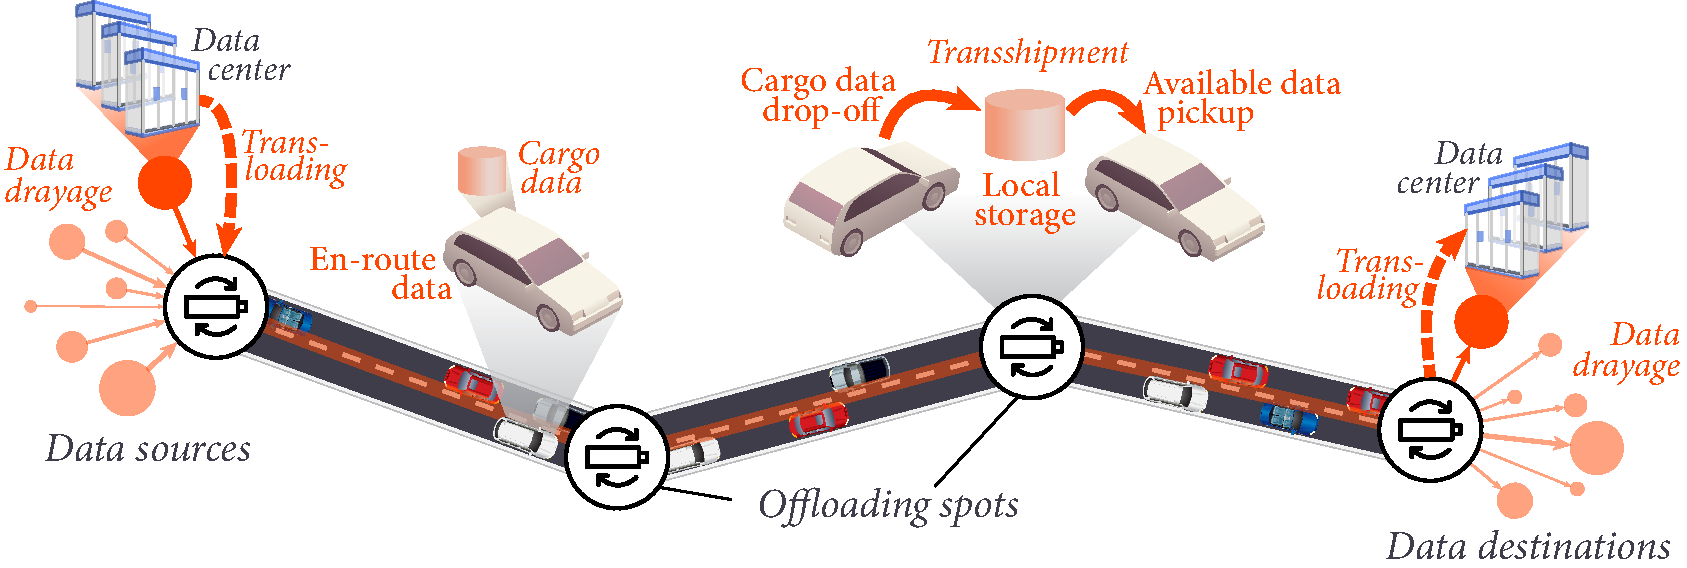
\includegraphics[width=0.95\columnwidth]{figures/taxonomy.pdf}
	\caption{Overview of the operations to offload large amounts of data over the road network.}
	\label{fig:offloading-operations}
\end{figure}

The flow of vehicles so equipped acts as a mechanical backhaul\index{mechanical backhaul} connecting a collection of offloading spots, as depicted in Figure~\ref{fig:offloading-operations}.
%The term \textit{offloading spot}\index{offloading spot|bb} refers to specific locations featured with storage capabilities where vehicles may be parked long and close enough as part of their routines. 
The term \textit{offloading spot} refers to a fixed device offering short- to medium-term data storage, located where vehicles stop for long periods of time as part of their travel route. Examples of such locations include on-street parking spots, parking lots, or gas stations. In the case of electric vehicles, the offloading spots may be located at the battery charging stations such as the ones operated worldwide by ChargePoint\footnote{\url{http://www.chargepoint.com/}}. Offloading spots are equipped with wireless communication interfaces to support short-range radio data exchanges with vehicles while stopped. 

%The offloading service we propose relies on the opportunistic use of private vehicles equipped with storage capacities in combination with a collection of fixed wireless data storage devices referred to as \textit{offloading spots}\index{offloading spot|bb} (as illustrated in Figure~\ref{fig:taxonomy}). Vehicles are equipped with one or more removable storage devices such as hard drives or other non-volatile solid-state drives. Each vehicle carries a \textit{cargo}\index{data cargo|bb} of data in their storage devices. 
%We assume that vehicles also embed a \acrfull{gps} that generates routes and guidance between a geographic location and a destination. The flow of vehicles so equipped acts as a mechanical backhaul\index{mechanical backhaul} connecting a collection of offloading spots. 

%Offloading spots remove the need of relying on the only vehicles making the trip all the way from the source to the destination of a data transfer. 

Offloading spots act as data relay exchange points where data is \textit{transloaded}\index{transloading} from a conventional data network to the closest offloading spot using a \textit{drayage}\index{drayage} system and stored until shipped to its destination by vehicles. Different techniques to implement a data drayage system are presented in Section~\ref{sec:discuss}. We take advantage of the parking time of the vehicle to opportunistically load data on or off their storage devices. 

Vehicles unload their data cargo while they are stopping at an offloading spot if they are heading in a different direction than the destination of the data they carry. The data is stored until transferred to a subsequent empty vehicle heading towards the intended destination. As a result, the data may be transferred on multiple vehicles following different trajectories before reaching its destination. Splitting the data path across different vehicles makes the transfers less vulnerable to hijacking attempts on vehicles. To mitigate the effect of vehicles changing their travel directions or having accidents, offloading spots load the same data on multiple vehicles, either at the first offloading spot or at each intermediate offloading spot.

The data is therefore ``hitchhiked'' hop-by-hop through the network of offloading spots before reaching its final destination. Transfers of offloaded data result from the vehicles' routine journeys interspersed with stops at the offloading spots as part of their line of travel. Offloading spots thus remove the need of relying on the only vehicles making the trip all the way from the source to the destination of a data transfer.

% motivations for the offloading spots

The data offloaded from conventional networks follows the same path as the flow of vehicles traveling the road segments connecting sequences of offloading spots. 
%As depicted in Figure~\ref{fig:offloading-operations}, multiple consecutive offloading spots may be involved if the data needs to be shipped across a large body of country before reaching geographically long distant destinations. 

%To avoid the need of relying on vehicles solely traveling all the way from the source to the destination of the data transfers, offloading spots act as data exchange relay points. Vehicles in contact with an offloading spot unload their cargo if heading to a different direction with the destination of the data transfer. The data is stored until transferred to a subsequent vehicle heading towards the intended destination.
%Given the increasing number of vehicles driven and miles traveled, large chunks of data can be offloaded from an infrastructure network such as the Internet. 
For each offloading demand, the road network path is determined by solving the vehicle flow allocation problem we formulate as a multi-commodity flow allocation model in Section~\ref{sec:revenue-maximization-model}.


% An existing allocation plan may be dynamically modified in case the vehicles change direction unexpectedly or to account for new data transfers as they arrive. The dynamic allocation method we describe is applied to flows of vehicles. Such a flow refers to the group of electric vehicles traveling in the same direction between two adjacent offloading spots. We do not consider the complete journey of each vehicle traveling the underlying road network. The scheduling of the data transfers (\ie the selection of the data to be piggybacked), and the security and privacy issues are out of the scope of this article. In section~\ref{sec:discussion}, we will discuss potential future directions for addressing these issues. 


\subsection{Business model, assumptions, and roles}
\label{sec:business-model}

\begin{figure}[h!]
    \centering
    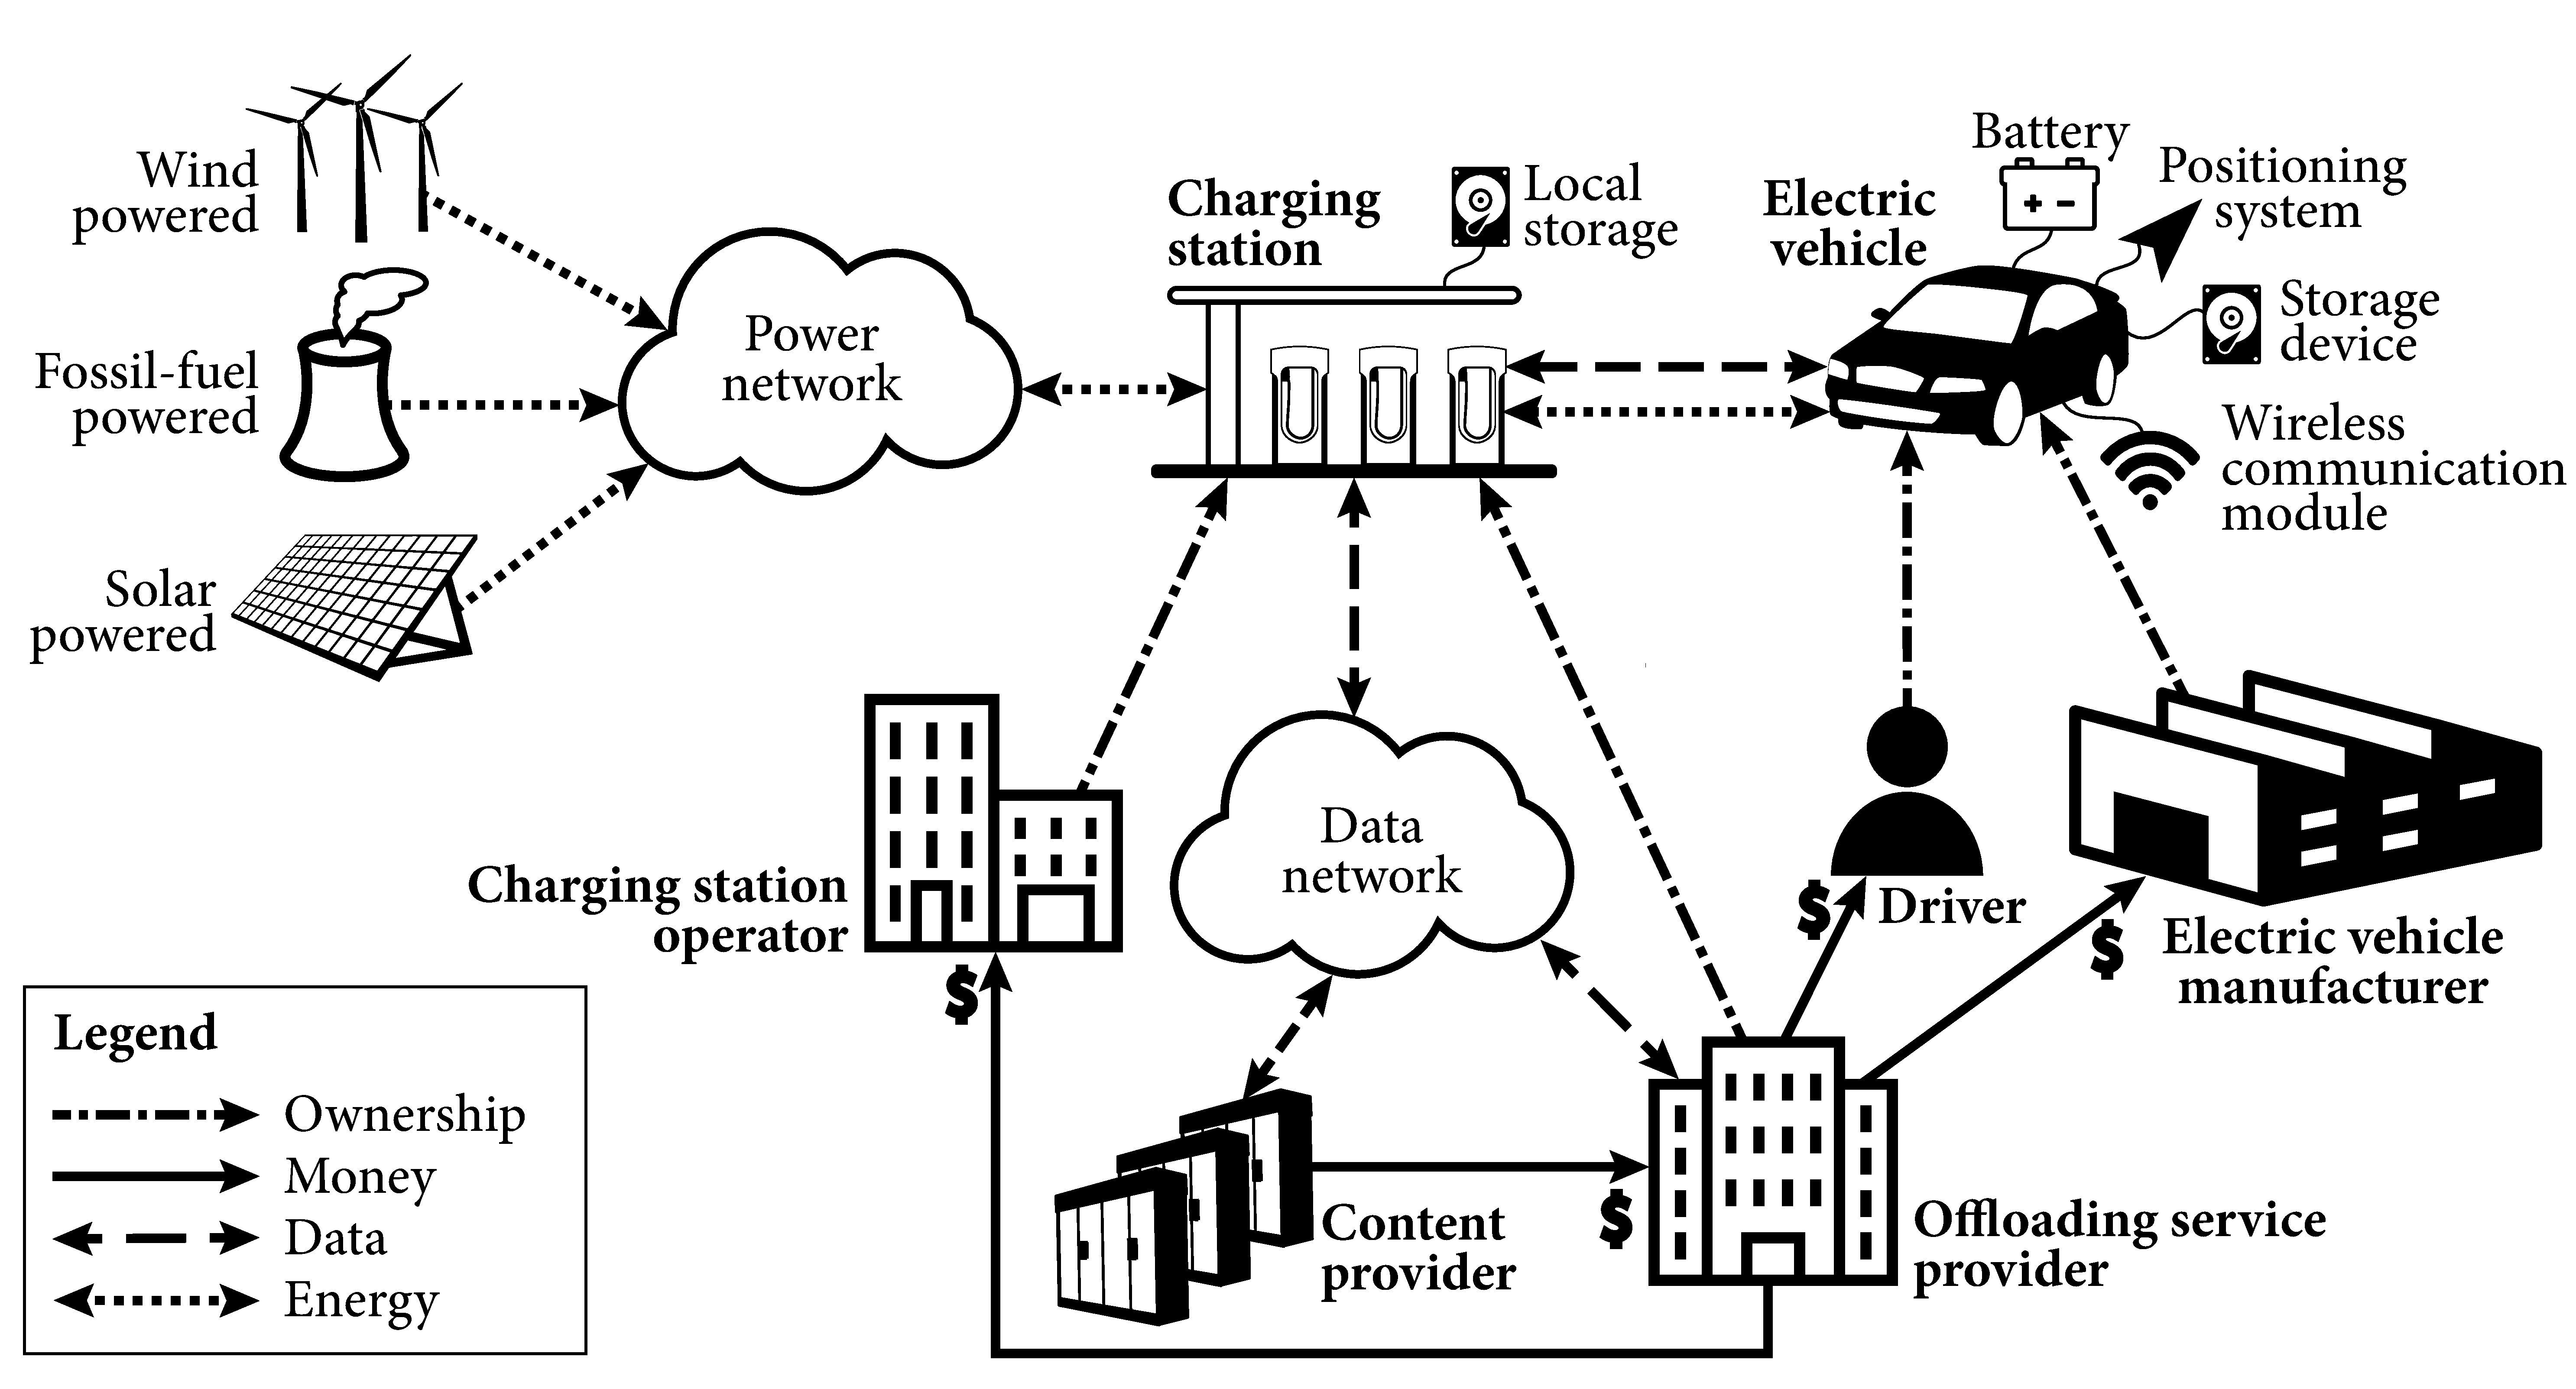
\includegraphics[width=0.9\textwidth]{figures/business-plan.pdf}
    \caption{Business model for the vehicular data offloading concept.}
    \label{fig:business-model}
\end{figure}

In this section, we present the business model we will use throughout this thesis. We represent the different actors involved in Figure~\ref{fig:business-model}, including (\textit{i}) \acrfullpl{ev} and their owners, (\textit{ii}) the offloading service provider (that can be the \acrshort{ev} manufacturers themselves), (\textit{iii}) the charging station operator, and (\textit{iv}) a content provider that operates multiple data centers. 

This model provides support for the modeling and analysis of our proposal in practical settings, including the driving range of \acrshortpl{ev} (\eg 320~km for the Tesla Model S) and the charging time of the batteries (\eg 20~minutes when charging at a Tesla supercharger\footnote{\url{https://www.tesla.com/supercharger}}). 

The electric vehicles are equipped with one or more data storage devices, such as hard drives or other non-volatile solid-state devices. 
%We assume that the content of the storage devices is not accessible by the drivers and the data encrypted when carried onto the vehicle. 
The term ``electric vehicle'' \acrshort{ev} refers to private vehicles propelled by one or more electric motors powered by a rechargeable battery. %Commercial vehicles may be part of a fleet owned or leased by a business or a governmental agency. 
%We assume that vehicles also embed one or more communication network interfaces. 
The charging stations act as \textit{offloading spots} where the data is seamlessly loaded on or unloaded from the onboard storage of the vehicles using short-range radio while they charge their battery. 

The offloading service provider, if different from the \acrshort{ev} manufacturers, proposes a ``get paid to drive'' program to the car owners. The service provider installs the storage devices and the vehicle owners receive a monthly fee or a discount on the cost of charging their vehicle in exchange for driving their normal routine. The discount rate is negotiated with the charging station operator (\eg ChargePoint who operates a worldwide network of \acrshort{ev} charging stations offering cloud-network services\footnote{\url{http://www.chargepoint.com/}}) and is calculated based on the driving pattern including coverage and mileage. If the \acrshort{ev} manufacturers take on the role of service provider, vehicles are equipped as standard with onboard storage and the service is provided without involving nor compensating the vehicles' drivers. The service provider charges the content provider for the amount of data to offload on the road network and shares the revenues with the charging station operator. 
%The offloading spots may also comprise battery swap stations where vehicles' memory implemented as removable devices are replaced with ready-to-ship devices so that vehicles can continue their travels without waiting for the data to be transferred.  

%Offloading spots act as intermediate data exchange relay points. Offloading spots enable the transshipment of data chunks as they can be dropped off for future pick-up by subsequent passing vehicles. The offloading spots transfer a data chunk on a charging vehicle using short-range radios. Every time a vehicle stops by an offloading spot, its destination is matched against the destination of the data chunk 

The offloading spots feature storage capabilities where data is transloaded from the conventional data network and temporarily stored 
%as \textit{data cargo}\index{data cargo} 
until transferred to a charging vehicle. 
%The content provider uses a border dray transfer system if the data originates from a distant repository, typically a wide-area data network such as the Internet connecting the content provider to the edge offloading spots. 
The service provider monitors the status of the offloading spots, which includes the amount of available storage and the destination of the data cargo in transshipment. To improve the forwarding decisions, the service provider also queries the stopping vehicles' positioning system to determine their current geographic destination. The historical locations are stored in a geographic location database managed by the service provider to help the offloading spots predict the remaining itinerary of the passing vehicles.  In Section~\ref{sec:discuss}, we present a list of probabilistic tools for inferring the remaining route of a vehicle knowing its navigation history and discuss the concerns regarding the drivers' and passengers' privacy.

%The service provider receives the demands to offload data transfers from the content provider. Each demand specifies the delay and bandwidth requirements for the corresponding data transfer. The service provider keeps track of the status of the offloading spots which include statistics about the charging vehicles. The offloading spot operator also reports information about the data cargo locally unloaded for later pickup. The service provider, which collects the information from the offloading spots, has an up-to-date view of the offloading infrastructure.

Upon receiving a demand to offload a data transfer from a content provider, the service provider computes the road network paths that can accommodate the data transfer requirements and how much data to allocate to each flow of vehicles. The road network path consists of a sequence of offloading spots, each configured with the list of actions to perform on each vehicle traveling in the direction of the next-hop offloading spot. Each action defines the behavior that the offloading spot operator needs to perform with the data belonging to the offloaded transfer. The corresponding data can either be already stored at the offloading spot or carried by the charging vehicle. Common actions include loading data cargo on or off the vehicles while charging their battery. The service provider defines these actions based on the information the offloading spot operator reports on the flows of vehicles passing through the offloading spots. For each vehicle stopping by an offloading spot, the offloading spot operator matches the destination of the vehicle against the data transfers currently offloaded on the road network and performs the actions as dictated by the service provider. 

\section{Road map reduction}
\label{sec:offloading-overlay}

Recall that our objective in this chapter is to assess the vehicular offloading concept by comparing the cost of using the offloading infrastructure including the offloading spots compared to the cost charged by Internet providers for transferring the same amount of data. We need to determine the routes followed by the vehicles carrying the data and offering the same performance as the one resulting of transferring the same amount of data on the Internet. 

To determine those routes, we present a revenue maximization model in Section~\ref{sec:revenue-maximization-model}. Before solving this model, we need to cope with the scale of the road network. The high degree of complexity of the road network's topology and the large number of vehicular trips make the revenue maximization problem computationally intractable.

In this section, we present a mapping algorithm that reduces the complexity of the road network. The output of our algorithm is an offloading overlay\index{offloading overlay|bb}, which refers to a logical representation that captures the characteristics of the road network. We provide a performance evaluation that measures the reduction factor resulting from the mapping algorithm by comparing the complexity of the offloading overlay over the actual road network.


\subsection{Road network}
\label{sec:road-network-characterization}

We represent the road network\index{road network|bb} by a directed graph $G^R=(N^R,\,L^R)$, where $N^R$ and $L^R$ denote the set of physical nodes and links, respectively. The set of nodes $N^R=N^J\cup N^S$ consists of two subsets: the set of road junctions ($N^J$) and the set of charging stations ($N^S$). A road junction refers to a location where vehicles can change their direction of travel. A link in the road network corresponds to a road segment connecting two adjacent junctions or a junction and a charging station. We consider the road segments and the traffic flowing in both directions homogeneous as they share the same profile in terms of capacity. For a road segment $(a,\,b)\in L^{R}$, let $v_{ab}$ be its nominal volume of vehicles (vehicles per unit of time), $c_{ab}$ be its capacity (vehicles per unit of time), and $t_{ab}(v_{ab})$ be its corresponding travel time that depends on the nominal volume of vehicles. 

We use publicly available datasets to characterize the road network. These datasets feature traffic volumes on the road segments, expressed in terms of \acrfull{aadt}\index{AADT}. \Acrshort{aadt} is the total volume of traffic traveling on a road segment in both directions for one year, divided by the number of days in the year. As a result, the capacity $c_{ab}$ of a road segment $(a,\,b)\in L^{R}$ are fixed to the \acrshort{aadt} value of the dataset for this road segment.


\subsection{Offloading overlay}
\label{sec:offloading-overlay-characterization}

\begin{wrapfigure}[15]{o}[0.7\marginparwidth]{7.5cm}
    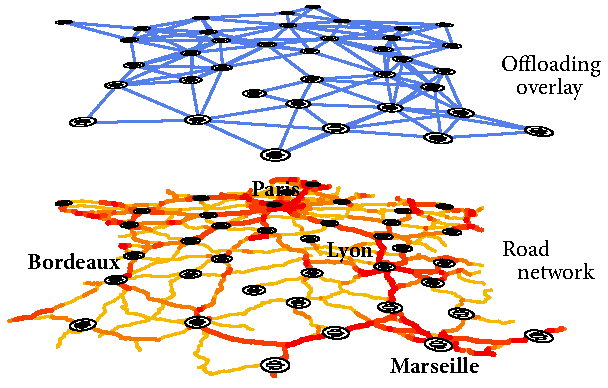
\includegraphics[width=7cm]{figures/France-overlay-1.pdf}
    \caption{The offloading overlay resulting from the deployment plan of battery charging stations acting as offloading spots for the French road network (the width and darkness of the road segments denote the vehicle density).}
    \label{fig:France-overlay}
\end{wrapfigure}
The offloading overlay\index{offloading overlay|bb} provides a logical representation\index{logical representation} of the road network. More specifically, the overlay mitigates the combinatorial explosion when enumerating the simple road paths in the road network, which becomes quickly intractable when the length of the paths increases. By providing a logical representation\index{logical representation} of the vehicle flows on the road paths connecting the offloading spots, the offloading overlay reduces the number of paths to enumerate. 
%and makes the data transfer allocation problem tractable.

We represent the offloading overlay by a directed graph $G^O=(N^O,\,L^O)$, where $N^{O}$ and $L^{O}$ denote the set of logical nodes and links, respectively. A logical node of $N^{O}$ is an offloading spot. A logical link of $L^{O}$ represents the road path (\ie a sequence of road segments) connecting two adjacent offloading spots in the road network. Note that, multiple road paths may connect two adjacent offloading spots, in which case, the logical link aggregates these paths. In Figure~\ref{fig:France-overlay}, we show an example of realization of an offloading overlay on top of the French road network. 

In the following Section~\ref{sec:characterization-offloading-overlay}, we characterize a logical link $(i,\,j)\in L^{O}$ with network quantities, that is by the weighted travel time $t(i,\,j)$, aggregated capacity $c(i,\,j)$ and data leakage $l(i,\,j)$. The data leakage refers to the loss rate on logical link $(i,\,j)\in L^{O}$ and accounts for the proportion of vehicles that fail to deliver the data to the next offloading spot $j$ because of errors in the prediction of the direction of the vehicle or accidents. We assume that offloading spots are not constrained by the amount of transfers they can serve and have the adequate storage capacity so that the overall service is stable. 


\subsection{Characterization of the offloading overlay} 
\label{sec:characterization-offloading-overlay}

In this section, we characterize the logical links of the offloading overlay into network quantities. The network quantities we consider in the following are relevant to solve the revenue maximization problem.

\paragraph{Travel time $t(i,\,j)$.} 
 The travel time $t{ab}$ of $(a,\,b)$ is given by the \acrfull{bpr} function defined as~\cite{BPR64}:

\begin{equation}
  \label{eq:BPR}
  t_{ab}(v_{ab})=t_{ab}(0)\left[1+\alpha\left(\frac{v_{ab}}{c_{ab}}\right)^{\beta}\right]\Comma
\end{equation}

\noindent where $\alpha$ and $\beta$ are \acrshort{bpr} parameters that depend on the road profile ($\alpha = 0.15$ minutes and $\beta = 4.0$ are typically used)~\cite{HCM00}.

We can deduce from Equation~\ref{eq:BPR} the travel time of physical path $p$, denoted $t_{p}$, which is the sum of all travel times of the road segments that compose the path (we do not consider any turning delays at junctions):

\begin{equation}
  \label{eq:path-delay}
  t_{p} = \sum_{(a,\,b)\in p} t_{ab}(v_{ab}).
\end{equation}

From Equation~\ref{eq:path-delay}, we deduce an expression of the average travel time\index{logical link!average travel time} $t(i,\,j)$ experienced on the $r$ physical paths between nodes $i$ and $j$, weighted by the road traffic flow $v_{p}$ on each path $p$:

\begin{equation}
  \label{eq:ovelray-link-delay}
  t(i,\,j) = \frac{\sum_{p\in S_{ij}} t_{p}\,v_{p}}{\sum_{p\in S_{ij}}v_{p}}\Comma
\end{equation}

\noindent where $S_{ij}$ is the set of all simple physical paths between $i$ and $j$ (\ie with no cycles in the path).

\paragraph{Capacity $c(i,\,j)$.}
The capacity\index{logical link!capacity} $c(i,\,j)$ of the overlay link $(i,\,j)\in L^{O}$ depends on the sum of the traffic flows $v_{p}$ of the simple paths between offloading spots $i$ and $j$ (\ie the number of vehicles per unit of time going from $i$ to $j$ on path $p$). The capacity $c(i,\,j)$ of the overlay link also depends on the market penetration ratio\index{market penetration ratio|bb} $\mathcal{M}$ of the vehicles participating in the data offloading and the storage size\index{storage size} $\mathcal{S}$ on each vehicle. We assume that all vehicles are equipped with a storage device of the same size $\mathcal{S}$.

\begin{equation}
  c(i,\,j) = \mathcal{M} \mathcal{S} \sum_{p\in \mathcal{P}^{ij}} v_{p}.
\end{equation}

In the performance evaluation presented in Section~\ref{sec:revenue-maximization-evaluation}, we derive the value of $v_{p}$ for each path $p$ from the French road network dataset. This dataset provides the real traffic counts in terms of \acrshortpl{aadt} for the road segments composing each path $p$.

\paragraph{Leakage $l(i,\,j)$.}
The leakage\index{logical link!leakage} $l(i,\,j)$ (comprised between 0 and 1) of logical link $(i,\,j)\in L^{O}$ represents the proportion of data that is lost between offloading spots $i$ and $j$. The leakage increases as more vehicles carrying data prematurely exit the road (\eg the vehicles may exit the highway before reaching the offloading spot or an accident may have occurred). The leakage depends on characteristics that are inherent to the physical paths mapped in the offloading overlay. Additionally, the leakage accounts for the errors inherent to the prediction of the direction of the vehicles when loading data at an offloading spot.

\section{Revenue maximization model}
\label{sec:revenue-maximization-model}

In this section, our objective is to assess the concept of vehicular offloading. The main step towards the feasibility of this concept can be stated as follows: Given a demand to offload a data transfer from a conventional data network, how does one select the road network paths and the flows of vehicles to match the demand requirements. 

We introduce the revenue maximization model\index{vehicle flow allocation problem!revenue maximization model|bb} that maximizes the cost-benefit of offloading traffic on the road network instead of using a conventional data network. We assume that the data is replicated in multiple copies each transferred over different vehicles to the next offloading spots. We devise two replication models resulting in two separate formulations of the revenue maximization models. 

\subsection{Offloading demands}
\label{sec:offloading-demands-feasibility}

An offloading demand\index{offloading demand} $d_{st}$ represents a request to offload a data transfer from a source offloading spot $s\in N^{O}$ to a target offloading spot $t\in N^{O}$. The demand is characterized by the amount of data $\beta_{st}$ and the deadline $\tau_{st}$ before which the transfer should be completed. Recall from Section~\ref{sec:offloading-overlay-characterization}, that we need to account for the vehicles that fail to reach the next offloading spot on time. Thus, each offloading demand is also characterized by a leakage tolerance $l_{st}$. We denote by $\mathcal{D}=\{d_{st}\}$ the matrix of the offloading demands indexed by the pairs of source and destination offloading spots $(s,\,t)$ of the corresponding data transfers. The leakage tolerance $0 < l_{st} \leq 1$ refers to the data loss ratio tolerated during the transfer on the road network, provided that the data is replicated at the source according to redundancy techniques (\eg Reed-Solomon or \acrshort{raid})~\cite{chen1994raid}, combined to the use of error correcting codes~\cite{macwilliams1977theory}. The leakage tolerance is consistent with the data encoding mechanism. Note that, $\beta_{st}$, the total amount of data to be transferred between $s$ and $t$, includes the redundant data introduced by the redundancy techniques. 

In the vehicle flow allocation model, $p$ denotes a logical simple path\index{logical path|bb} (\ie without any cycles) defined as the ordered list of offloading spots connected by logical links. $\mathcal{P}_{st}$ denotes the set of all logical simple paths from $s$ to $t$. We characterize the logical paths by the travel time $t(p)$ and the data flow (throughput) $f(p)$ allocated on logical path $p\in\mathcal{P}_{st}$ for a given offloading demand $d_{st}$ resulting from the vehicle flow allocation problem. The logical path travel time corresponds to the average time it takes to transfer one data cargo from one extremity of the path to the other. 


\subsection{Replication models}
\label{sec:replication-models}

We assume that the sequence and the properties of the links comprising the path followed by a data transfer remain unchanged for the time of the observation. We consider that offloading spots undertake two different behaviors when incoming vehicles unload their data cargo:

\begin{itemize}

	\item \textbf{Local replication (\textit{rep}).}\index{reliability!replication model!local replication} This model assumes that all offloading spots replicate data on multiple outgoing vehicles. For a given offloading demand $d_{st}$ and for each adjacent offloading spot $j$, offloading spot $i$ replicates data $\rho_{st}(i,\,j)$ times vehicles traveling on logical link $(i,\,j)\in L^{O}$ (\ie the same data is loaded onto $\rho_{st}(i,\,j)$ vehicles heading to $j$). This logical link is characterized by the leakage $l(i,\,j)$. The amount of replication needed is calculated such that it satisfies the leakage tolerance $l_{st}$ of the offloading demand. 

	\item \textbf{Source replication (\textit{nrep}).}\index{reliability!replication model!source replication} The second model assumes that none of the offloading spots replicate data on the outgoing vehicles, except at the source offloading spot. It takes into account the combination of the leakage on the logical links that compose logical path $p$, denoted by $l_{p}(i,\,j)$ for the resulting leakage at logical link $(i,\,j)$. Here, we assume the source can characterize the entire paths to be allocated using traffic forecasting techniques before the transfer happens~\cite{de2011modelling,sheffi1985urban}. For path $p$ and demand $d_{st}$, the source offloading spot $s$ replicates the data $\rho_{st}(p)$ times such that it satisfies the leakage tolerance $l_{st}$ of the offloading demand. 

\end{itemize}

\subsection{Cost model} 

We aim to measure the cost-benefit\index{cost model|bb} of offloading data over a solution relying on conventional data networks when delivering the same amount of data. We consider a offloading demand $d_{st}$ characterized by the amount of data to transfer $\beta_{st}$ and the transfer duration $\tau_{st}$ we target. Our model describes the cost-benefit of a data transfer, defined as the difference between the price charged by an \acrfull{isp} for transferring $\beta_{st}$ within $\tau_{st}$, and the operational costs induced by transferring data with the offloading infrastructure. In the following, we define the Internet-based price and the operational costs.

\begin{itemize}
	
	\item \textbf{Internet-based cost.}\index{cost model!Internet-based cost} $\gamma_{st}$ is the unit cost to send a bit of data from $s$ to $t$ over the legacy Internet (\eg a leased line between $s$ and $t$). As an example, $\gamma_{st}$ may vary in function of the distance between $s$ and $t$. Without loss of generality, we assume that $\gamma_{st}$ is linear with the volume of data transferred. $\gamma_{st}$ may also be seen as the savings one can achieve by using our offloading infrastructure instead of an Internet-based solution.
	
	\item \textbf{Operational costs.}\index{cost model!operational costs} $\alpha_{i}$ is the operational cost needed for the maintenance of the storage facility at offloading spot $i$, as well as the financial compensations given to the drivers of the vehicles involved in the data offloading. We assume $\alpha_{i}$ is also linear with the volume of data exchanged at offloading spot $i$. The value of $\alpha_{i}$ depends on the replication model we consider. $\alpha^{\text{rep}}_{i}$ corresponds to the local replication model and $\alpha^{\text{nrep}}_{i}$ corresponds to the source replication model. The local replication model will require the data to be stored for longer periods of time. Each copy is held until it can be transferred to a vehicle matching the destination of the data. Hence, the need for extra storage facilities will induce higher operational costs for the local replication model $\alpha^{\text{rep}}_{i}$, compared to the source one $\alpha^{\text{nrep}}_{i}$.
	
\end{itemize}

Note that we do not explicitly consider the \acrfull{capex} to deploy the infrastructure required to offload data over the road network. The \acrshort{capex} includes the storage facilities at the offloading spots and the storage devices installed on the vehicles. Instead, we consider the infrastructure already deployed and exploited by the offloading spot operator (\eg the charging station operator\index{charging station operator}). Hence, the \acrshort{capex} costs are amortized and thus accounted for in the operational costs we consider.

In the following, we present our revenue maximization model\index{vehicle flow allocation problem!revenue maximization model} as a \acrlong{lp} model derived from a \acrlong{mcf} allocation model\index{multi-commodity flow allocation}. The model maximizes the overall cost-benefit of offloading the entire set of demands $\mathcal{D}$ between each pair of (source, destination). Our cost model constraints the objective by both the delay tolerance $\tau_{st}$ and the capacity $c(i,\,j)$ of the logical links. We summarize in Table~\ref{tab:main-variables-feas} the variables we use in our model.

\begin{table}[!t]
    \caption{Table of notations for the revenue maximization problem.}
    % increase table row spacing, adjust to taste
    \renewcommand{\arraystretch}{1.1}
    \centering
    % Some packages, such as MDW tools, offer better commands for making tables
    % than the plain LaTeX2e tabular which is used here.
    {\footnotesize
    \begin{tabular}{c|l}
        \textbf{Variable} & \textbf{Meaning}\tabularnewline
        \hline 
        $d_{st}$ & Offloading demands between source $s$ and destination $t$\tabularnewline
        $\tau_{st}$ & Delay tolerance of demand $d_{st}$\tabularnewline
        $l_{st}$ & Leakage tolerance of demand $d_{st}$\tabularnewline
        $\beta_{st}$ & Amount of data transferred for demand $d_{st}$\tabularnewline
        $\mathcal{P}_{st}$ & Set of simple paths between $s$ and $t$ on the offloading overlay\tabularnewline
        $\mathcal{S}$ & Storage capacity of the vehicles (cargo size)\tabularnewline
        $\mathcal{M}$ & Market penetration ratio\tabularnewline
        $\gamma_{st}$ & Internet-based cost for demand $d_{st}$\tabularnewline
        $\alpha_{i}$ & Operational cost at offloading spot $i$\tabularnewline
        $\delta_{i}$ & Waiting time at offloading spot $i$ (to load data)\tabularnewline
        $f(p)$ & Flow allocated on logical path $p$\tabularnewline
        $t(p)$ & Travel time of logical path $p$\tabularnewline
        $\rho_{st}(p)$ & Replication factor for demand $d_{st}$ on path $p$\tabularnewline
        $\rho_{st}(i,\,j)$ & Replication factor for demand $d_{st}$ on link $(i,\,j)\in L^{O}$\tabularnewline
        $t(i,\, j)$ & Weighted travel time of logical link $(i,\, j)\in L^{O}$\tabularnewline
        $c(i,\, j)$ & Capacity of logical link $(i,\, j)\in L^{O}$\tabularnewline
        $l(i,\, j)$ & Leakage of logical link $(i,\, j)\in L^{O}$\tabularnewline
        $l_{p}(i,\, j)$ & Combined leakage of logical path $p$ at link $(i,\, j)\in L^{O}$\tabularnewline
    \end{tabular}}
    \label{tab:main-variables-feas}
\end{table}

In the following, we formulate the revenue maximization problem using the offloading overlay with a linear programming model that aims at maximizing the cost-benefit of offloading data over the road network. We consider a snapshot of the system, \ie a state of a system characterized by given parameters valid for the duration of the data transfers (offloading demands, road traffic flows, travel time and  leakage on logical links).

\section{Data offloading revenue maximization}
\label{sec:revenue-maximization}

In Section~\ref{sec:revenue-maximization-model}, we described the revenue maximization model we consider that maximizes the cost-benefit of offloading data transfers on the road network. Here, we present the two revenue maximization models which differ depending on the data replication models used for the data transfers.

The travel time\index{logical path!travel time} $t(p)$ experienced on logical path $p\in \mathcal{P}$ is the sum of the travel times $t(i,\,j)$ on the logical links of $p$ and the waiting time $\delta_{i}$ at each intermediate offloading spot on the path:
\begin{equation}
    t(p) = \sum_{(i,\,j)\in p} \big(t(i,\,j) + \delta_{i}\big).
    \label{eq:feas-logical-path-travel-time}
\end{equation}

For the same offloading demand, the transfer of an amount of data $\beta_{st}$ is constrained by the delay tolerance $\tau_{st}$ and does not depend on the data replication model. Hence, the delay constraint is the same for both models. The delay to transfer $\beta_{st}$ between $s$ and $t$ is the sum of the duration to transfer this quantity over all logical paths between $s$ and $t$ and the average travel time experienced on these paths, weighted by the flow on each path. The delay constraint is expressed as:

\begin{equation}
    \frac{\sum_{p\in \mathcal{P}_{st}}f(p)t(p)}{\sum_{p\in \mathcal{P}_{st}}f(p)} + \frac{\beta_{st}}{\sum_{p\in \mathcal{P}_{st}}f(p)} \leq \tau_{st}.
    \label{eq:delay-constraint-0}
\end{equation}

Equation~\ref{eq:delay-constraint-0} is not a linear expression, which can lead to some difficulties to solve the linear optimization problem. But it can be rewritten as the following linear expression:

\begin{equation}
    \sum_{p\in \mathcal{P}_{st}}f(p)\left(\tau_{st} - t(p)\right) \geq \beta_{st}.
    \label{eq:delay-constraint}
\end{equation}


\subsection{The ``local replication'' model}
\label{sec:rep-model}

Recall that, in this model\index{reliability!replication model!local replication}, every offloading spots store and replicate data. Consider a given offloading demand $d_{st}$ with leakage tolerance $l_{st}$ and $p\in\mathcal{P}_{st}$ a path between $s$ and $t$. If $\rho_{st}(i,\,j)f(p)$ data is transmitted on overlay link $(i,\,j)\in p$, $f(p)$ data is received at destination offloading spot $j$. Here, the replication factor $\rho_{st}(i,\,j)$ is calculated by each offloading spot $i$ that sends data to remote offloading spot $j$ on logical link $(i,\,j)\in L^{O}$ as a function of $l_{st}$ and $l(i,\,j)$ as follows:

\begin{equation}
    l(i,\,j)^{\rho_{st}(i,\,j)}\leq l_{st} \implies
    \rho_{st}(i,\,j) \geq \frac{\log(l_{st})}{\log(l(i,\,j))}\cdot
\end{equation}

The flow on logical link $(i,\,j)\in L^{O}$ is expressed as the sum of all flows sent by offloading spot $i$ to offloading spot $j$ on logical link $(i,\,j)$ for offloading demand $d_{st}$. The flow is constrained by the capacity of the logical link $c(i,\,j)$:

\begin{equation}
    \sum_{s,\,t\in \mathcal{D}\vphantom{\mathcal{P}_{st}}} \sum_{\substack{p\in \mathcal{P}_{st}\\p\ni (i,\,j)}} \rho_{st}(i,\,j)\, f(p) \leq c(i,\,j).
\end{equation}

Recall that, the cost-benefit is expressed as the difference between the cost of an Internet-based service (using the cost factor $\gamma^{st}$) and the operational costs of the offloading infrastructure (costs $\alpha_{i}^{\text{rep}}$ at each offloading spot $i$). Our objective is to maximize the cost-benefit of offloading data, expressed as follows:

\begin{equation}
    \label{eq:total-revenue-obj}
    \sum_{s,\,t\in \mathcal{D}\vphantom{N^{O}}}\beta_{st}\gamma_{st} - \sum_{i\in N^{O}\vphantom{N^{O}}}\alpha_{i}^{\text{rep}} \sum_{p\ni i\vphantom{N^{O}}}f(p).
\end{equation}

One can note that the contribution to the value of Equation~\ref{eq:total-revenue-obj} of each $f(p)$ is negative. Besides, the only lower bonding constraint on $f(p)$ is Equation~\ref{eq:delay-constraint}, which can be interpreted as a requirement on the total flow between each pair $(s,\,t)$. Therefore, maximizing the cost-benefit tends to minimize $\sum f(p)$, and Equation~\ref{eq:delay-constraint} is tight at optimality. It is thus possible to replace $\beta_{st}$ in Equation~\ref{eq:total-revenue-obj} as follows.

% We note that if Equation~\ref{eq:total-revenue-obj} is optimal (i.e., maximize), then Equation~\ref{eq:delay-constraint} becomes an equality since the quantities $\beta_{st}$ are constrained only in the latter equation and $\gamma^{st} > 0$. Now, if we consider an equality instead of an inequality for the delay constraint Equation~\ref{eq:delay-constraint}, when replacing $\beta_{st}$ with its expression, the maximal gross margin objective can be rewritten as:

\begin{equation}
    \sum_{s,\,t\in \mathcal{D}\vphantom{\mathcal{P}_{st}}} \sum_{p\in \mathcal{P}_{st}\vphantom{\mathcal{P}_{st}}} f(p) {\left[\gamma_{st}\big(\tau_{st} - t(p)\big) - \alpha^{\text{rep}}(p)\right]},
    \label{eq:total-revenue-obj-1}
\end{equation}

\noindent where $\alpha^{\text{rep}}(p) = \sum_{i\in p}\alpha_{i}^{\text{rep}}$.

In Equation~\ref{eq:total-revenue-obj-1}, if $\gamma^{st}\big(\tau_{st} - t(p)\big) - \alpha^{\text{rep}}(p)$ is negative, then $f(p)$ is null (objective function decreases otherwise). Hence, from Equation~\ref{eq:total-revenue-obj-1}, we have:

\begin{equation}
    t(p) + \frac{\alpha^{\text{rep}}(p)}{\gamma_{st}} \geq \tau_{st} \implies f(p) = 0.
    \label{eq:cutoff-rep}
\end{equation}

\noindent Since Equation~\ref{eq:cutoff-rep} is a weight on the logical paths (resulting from the weights of the logical links) that depends only on the offloading overlay, we can narrow the search space of the paths that do not satisfy Equation~\ref{eq:cutoff-rep}. Finally, the formulation can be reduced to the cost-benefit maximization objective subject to the capacity constraint on each logical link $(i,\,j)$:

\begin{flalign*}
    & \text{Maximize } \sum_{s,\,t\in \mathcal{D}\vphantom{\mathcal{P}_{st}}}\sum_{p\in \mathcal{P}_{st}\vphantom{\mathcal{P}_{st}}} f(p)\psi_{st}^{\text{rep}}(p), &
    \shortintertext{subject to}
    & \sum_{s,\,t\in \mathcal{D}\vphantom{\mathcal{P}_{st}}} \sum_{\substack{p\in \mathcal{P}_{st}\\p\ni (i,\,j)}} \rho_{st}(i,\,j) f(p) \leq c(i,\,j) \qquad \forall (i,\,j)\in L^{O},
\end{flalign*}

\noindent where $\psi_{st}^{\text{rep}}(p)=\gamma_{st}\big(\tau_{st}-t(p)\big)-\alpha^{\text{rep}}(p)$ can be considered as a weight on logical path $p\in\mathcal{P}_{st}$.

\subsection{The ``source replication'' model}
\label{sec:nrep-model}

In this model\index{reliability!replication model!source replication}, data is replicated at the source offloading spot to satisfy the leakage tolerance $l_{st}$ of the offloading demand $d_{st}$. We assume again that the source can characterize all logical simple paths between the source $s$ and the destination $t$ so it can compute the resulting path leakage $l_{p}(i,\,j)$ for every logical link $(i,\,j)$ in logical path $p\in\mathcal{P}_{st}$. 

We denote by $l_{p}(i,\,j)$ the multiplied leakage experienced at logical link $(i,\,j)\in L^{O}$ on logical path $p$. If $p=(i_{0},\,\dotsc,\,i_{n}),\,i_{k}\in N^{O}$ is a logical simple path between $i_{0}$ and $i_{n}$, then for all $0 \leq k < n$, the leakage $l_{p}(i_{k},\,i_{k+1})$ at logical link $(i_{k},\,i_{k+1})\in L^{O}$ is expressed as:

\begin{equation}
    l_{p}\left(i_{k},\, i_{k+1}\right)=1-\prod_{j=1}^{k}\big(1 - l\left(i_{j-1},\, i_{j}\right)\big),
\end{equation}

\noindent where $0 \leq k < n$. Since the source $s$ knows the attributes of the logical path $p$, it may deduce the replication factor $\rho_{st}(p)$ introduced in Section~\ref{sec:replication-models}. For offloading demand $d_{st}$ allocated on logical path $p=(s,\,i_{1},\,\dotsc,\,i_{n-1},\,t)\in\mathcal{P}_{st}$, the replication factor $\rho_{st}(p)$ is calculated by the source $s$ as follows:

\begin{equation}
    l_{p}(i_{n-1},\,t)^{\rho_{st}(p)} \leq l_{st} \implies
    \rho_{st}(p) \geq \frac{\log(l_{st})}{\log(l_{p}(i_{n-1},\,t))}\cdot
\end{equation}

For each logical link $(i,\,j)\in L^{O}$, the capacity constraint limits to the logical link capacity $c(i,\,j)$ the amount of assigned flows $f(p)$ for each path $p$ that go through the logical link $(i,\,j)$ with the proportion of leftover flow at the logical link $1 - l_{p}(i,\,j)$ and replication factor $\rho_{st}(p)$ for offloading demand $d_{st}$:

\begin{equation}
    \sum_{s,\,t\in \mathcal{D}\vphantom{\mathcal{P}_{st}}} \sum_{\substack{p\in \mathcal{P}_{st}\\p\ni (i,\,j)}} \rho_{st}(p) \big(1 - l_{p}(i,\,j)\big) f(p) \leq c(i,\,j).
\end{equation}

As in the local replication model, the cost-benefit is expressed as the difference of the cost of an Internet-based service (with the cost factor $\gamma_{st}$) and the operational cost of the offloading infrastructure $\alpha^{\text{nrep}} \ll \alpha^{\text{rep}}$. In this model, we also aim at maximizing the cost-benefit of offloading data:

\begin{equation}
    \sum_{s,\,t\in \mathcal{D} \vphantom{\mathcal{P}_{st}}}\left[\beta_{st}\gamma_{st} - \smashoperator{\sum_{i\in N^{O} \vphantom{\mathcal{P}_{st}}}} \alpha_{i}^{\text{nrep}} \smashoperator[l]{\sum_{j\in N(i) \vphantom{\mathcal{P}_{st}}}} \smashoperator[r]{\sum_{\substack{p\in \mathcal{P}_{st}\\p\ni (i,\,j)}}} \rho_{st}(p) \big(1 {-} l_{p}(i,\,j)\big) f(p)\right].
\label{eq:maximization-obj-0}
\end{equation}

If Equation~\ref{eq:delay-constraint} is optimal, then it turns into an equality since it is the only equation that constrains $\beta_{st}$, given that $\gamma^{st} > 0$. Therefore, we can rewrite Equation~\ref{eq:maximization-obj-0} as follows:

\begin{equation}
    \sum_{s,\,t\in \mathcal{D} \vphantom{\mathcal{P}_{st}}} \smashoperator[r]{\sum_{p\in\mathcal{P}_{st}\vphantom{\mathcal{P}_{st}}}} f(p) \negmedspace \left[\gamma_{st}\big(\tau_{st} {-} t(p)\big) {-} \negmedspace \smashoperator{\sum_{\substack{p\in \mathcal{P}_{st}\\p\ni (i,\,j)}}}\alpha_{i}^{\text{nrep}} \! \rho_{st}(p) \big(1 {-} l_{p}(i,\,j)\big)\right].
\label{eq:maximization-obj}
\end{equation}

In Equation~\ref{eq:maximization-obj}, we note that if the factor of $f(p)$ is negative, then, since $f(p)\geq 0$, the objective function decreases, making it non-optimal. Thus, if the factor of $f(p)$ is negative, the flows $f(p)$ must be null. From the former Equation~\ref{eq:maximization-obj}, we have:

\begin{equation}
    t(p) + \frac{\rho_{st}(p)}{\gamma_{st}} \smashoperator{\sum_{\substack{p\in \mathcal{P}_{st}\\p\ni (i,\,j)}}} \alpha_{i}^{\text{nrep}} \big(1 - \mathcal{L}_{p}(i,\,j)\big) \geq \tau_{st} \implies f(p) = 0.
    \label{eq:cutoff-nrep}
\end{equation}

\noindent Similar to Equation~\ref{eq:cutoff-rep}, Equation~\ref{eq:cutoff-nrep} is a weight on the logical paths (although, not resulting from the weights of the logical links) that only depend on the offloading overlay; we can narrow the search space of the paths that do not satisfy Equation~\ref{eq:cutoff-nrep}.

Finally, the formulation can be reduced to the total revenue maximization objective subject to the capacity constraint on each logical link $(i,\,j)\in L^{O}$:

\begin{flalign*}
    &\text{Maximize }\sum_{s,\,t\in \mathcal{D}\vphantom{\mathcal{P}_{st}}}\sum_{p\in \mathcal{P}_{st}\vphantom{\mathcal{P}_{st}}} f(p)\psi_{st}^{\text{nrep}}(p), &
    \shortintertext{subject to}
    & \sum_{s,\,t\in \mathcal{D}\vphantom{\mathcal{P}_{st}}} \smashoperator[r]{\sum_{\substack{p\in \mathcal{P}_{st}\\p\ni (i,\,j)}}} \rho_{st}(p) \big(1 - l_{p}(i,\,j)\big) f(p) \leq c(i,\,j) \qquad \forall (i,\,j)\in L^{O}, & 
    \shortintertext{where}
    &\psi_{st}^{\text{nrep}}(p)=\gamma_{st}\big(\tau_{st}-t(p)\big)- \smashoperator{\sum_{\substack{p\in \mathcal{P}_{st}\\p\ni (i,\,j)}}} \alpha^{\text{rep}}(p)\rho_{st}(p)\big(1 - \mathcal{L}_{p}(i,\,j)\big). &
\end{flalign*}

The amount of data transferred $\beta_{st}$ within the delay tolerance $\tau_{st}$ imposed by offloading demand $d_{st}$ is deduced from Equation~\ref{eq:delay-constraint}:

\begin{equation}
    \beta_{st} = \sum_{p\in\mathcal{P}_{st}} f(p)\big(\tau_{st} - t(p)\big).
    \label{eq:total-transfer}
\end{equation}

We can finally obtain from Equation~\ref{eq:total-transfer} the average throughput of offloading demand $d_{st}$ by dividing the amount of data $\beta_{st}$ by the duration of the transfer $\tau_{st}$.

\clearpage
\section{Performance evaluation on the French road network}
\label{sec:revenue-maximization-evaluation}

In this section, we evaluate the performance of the revenue maximization problem by comparing the throughput resulting from the cost-benefit maximization under varying parameters, including the Internet-based cost, delay tolerance, leakage tolerance, and logical link leakage.

\subsection{Dataset of French road traffic}

\begin{wrapfigure}[17]{o}[0.7\marginparwidth]{7cm}
    \vspace{-20pt}
    \centering
    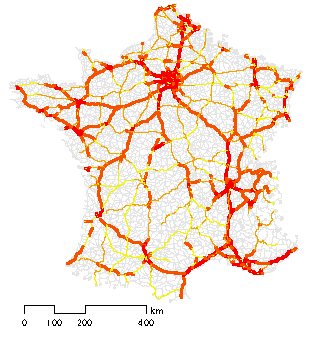
\includegraphics[width=6.8cm]{figures/france-dataset.pdf}
    \caption{Dataset showing the \acrfull{aadt} of the major roads of France in 2011. The road segments have a darker shade when \acrshort{aadt} is higher.}
    \label{fig:france-dataset}
\end{wrapfigure}
We use a dataset\index{French road network} collected in 2011 featuring the \acrfull{aadt}\index{AADT} of the major roads in France covering a combined distance of 20,000~km\footnote{\acrshort{entd}~---~Census of the road traffic on the French roads in 2011 (in French): \url{http://tinyurl.com/otfbewv}}.  The traffic volumes are collected using strategically located automatic traffic recorders. The different thickness and shades of red of the road segments depicted in Figure~\ref{fig:france-dataset} reflect the traffic counts given by the \acrshortpl{aadt}. The graph consists of 3,310 edges covering over 20,000~km of roads. 

\subsection{Planning of the network of charging stations}
\label{sec:charging-station-network}

We consider a network of charging stations similar to the one Tesla\index{Tesla} is currently rolling out in Europe and North America\footnote{\url{https://www.Teslamotors.com/supercharger}}. This network of stations helps electric vehicles face the problem of limited autonomy and achieve long distance travels. Recall that the offloading process will take place in these stations in a transparent manner to the driver. Since there was no such a network in France at the beginning of this thesis, we plan a simple yet realistic network of stations that covers the major roads of France. To plan such a network of stations, we consider a facility-allocation problem\index{facility-allocation problem} that minimizes the number of facilities to allocate, a problem we adapted from the maximal covering location problem~\cite{church1974maximal}. The problem takes demand points and candidate locations as inputs:
\begin{itemize}

	\item The demand points are the 9,555 cities of France with a population greater than 1,000.
   
	\item The candidate locations are the 1,024 Total gas stations, a French oil company.\footnote{\url{http://www.total.fr/mes-deplacements/outils-en-mobilite/export-gps-stations.html} (in French)}

\end{itemize}

The facility-allocation algorithm selects the stations such that a maximum demand points are allocated to the charging stations within a range of 150~km, while minimizing the number of chosen stations. We assume that vehicle ownership is uniform throughout the territory~---~we can then weight the cities by their population. The chosen stations are allocated at most 150~km away from each other. This is enough for a vehicle with an autonomy of 300~km to reach the next closest station or return to the same station without depleting its battery. Finally, we assume that the stations have a capacity that suits the demand such it avoids any waiting time at the stations. The waiting time is then restricted to the service time, which corresponds to the duration of the battery charge.

The resulting allocation outputs 38 stations scattered on the French road network, as shown in Figure~\ref{fig:France-location-allocation}. We note that the stations are mainly allocated near major cities, as the demand from urban areas is higher than from rural areas.

\begin{figure}[ht]
    \centering
    \begin{subfigure}[t]{0.47\columnwidth}
            \centering
            % \raisebox{.2\textwidth}{
            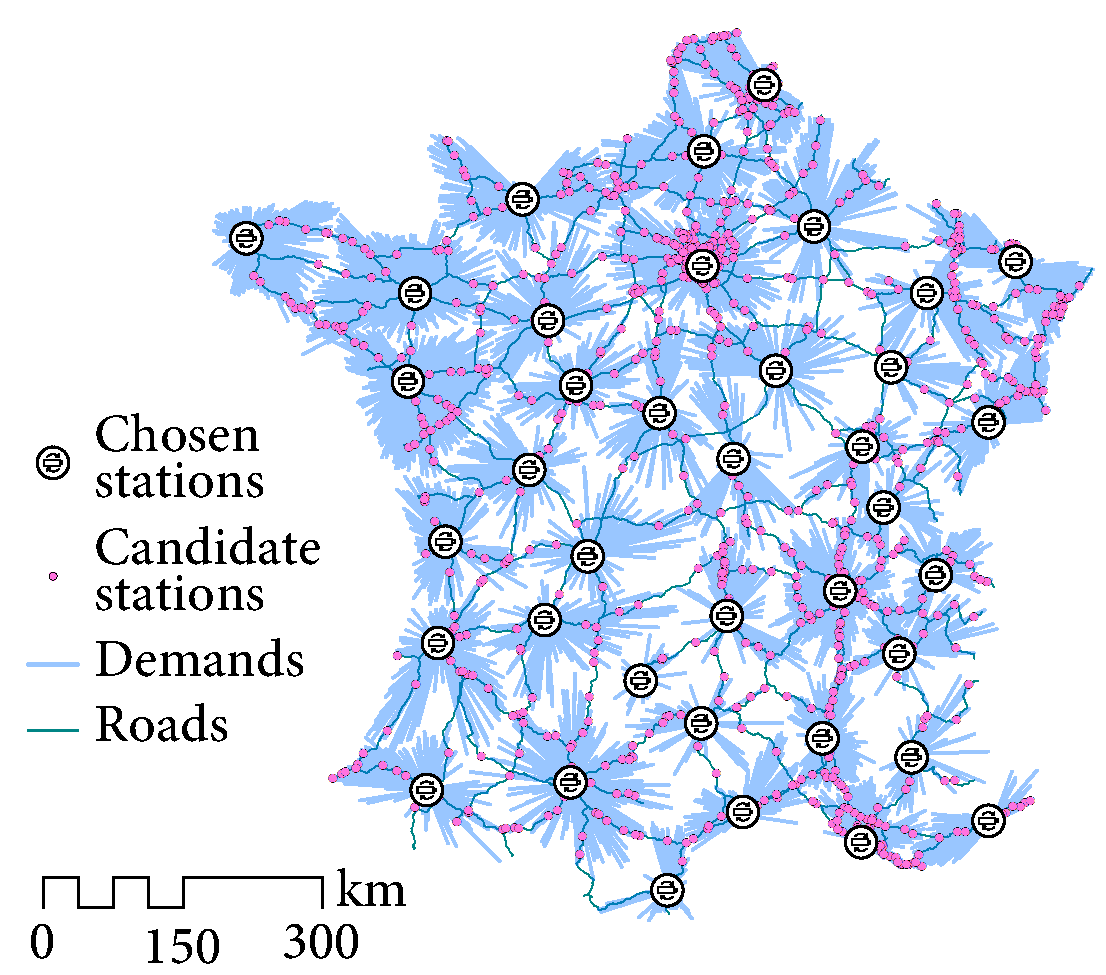
\includegraphics[width=0.98\textwidth]{figures/France-allocation-charging-stations.pdf}
            % }
            \caption{Charging station allocation over the French road network. The big dots are the chosen stations, the small dots are the candidate stations, and the lines represent the allocated demands to the chosen stations.}
            \label{fig:France-location-allocation}
    \end{subfigure}%
    \quad %add desired spacing between images, e. g. ~, \quad, \qquad etc.
      %(or a blank line to force the subfigure onto a new line)
    \begin{subfigure}[t]{0.5\columnwidth}
            \centering
            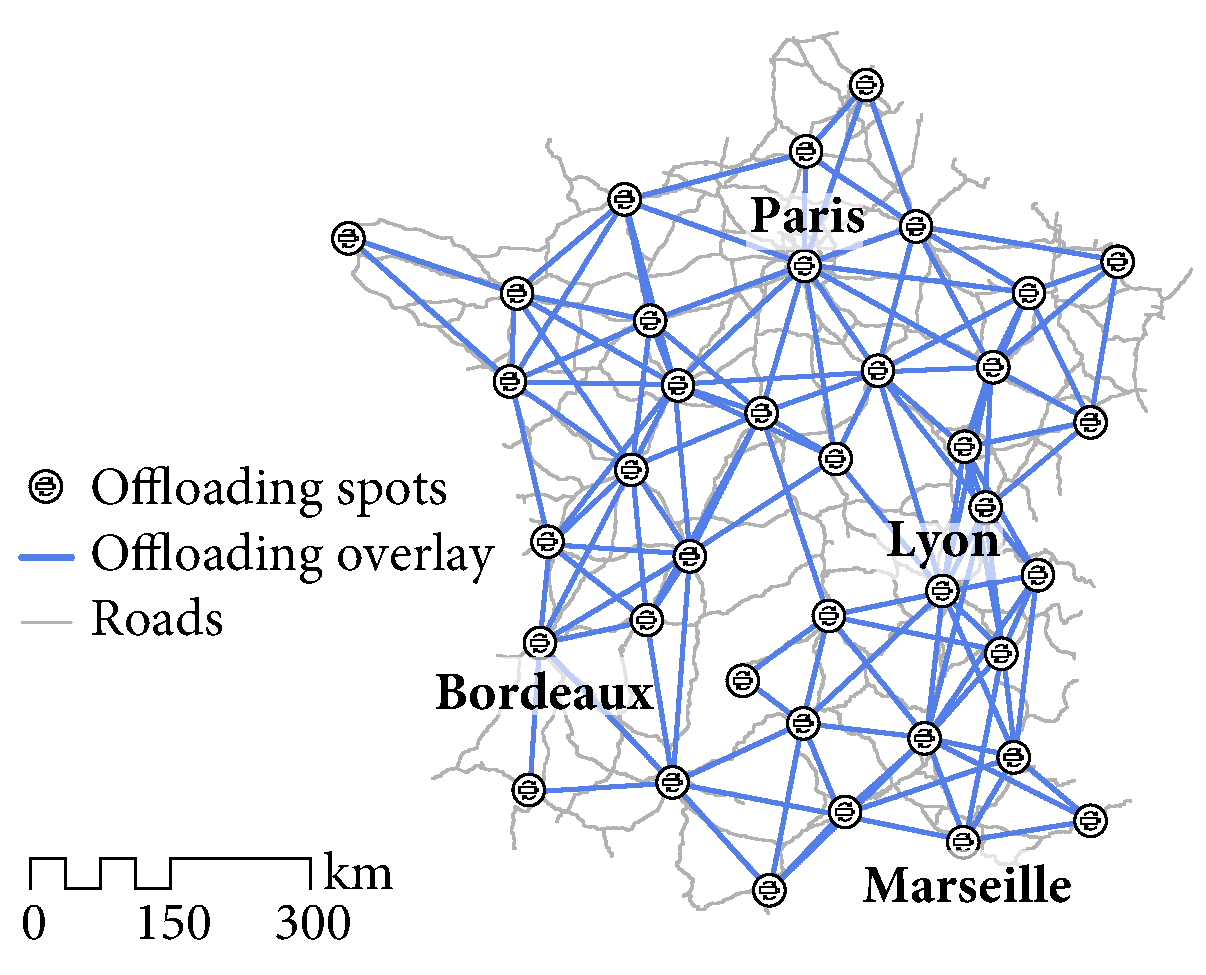
\includegraphics[width=\textwidth]{figures/France-overlay-wo-capacity.pdf}
            \caption{Resulting offloading overlay built on to of the road network of France. The offloading spots are those represented in Figure~\ref{fig:France-location-allocation}.}
            % (deduced from the AADT values)
            \label{fig:France-overlay-wo-capacity}
    \end{subfigure}
    \caption{Facility-allocation result and offloading overlay. The big dots are the chosen stations.}
\end{figure}

In the following, we first provide this characterization with conservative assumptions on the road traffic between the offloading spots. Second, we run the revenue maximization problem we introduced in Section~\ref{sec:revenue-maximization-model} on the offloading overlay for three large-scale data transfers. 


\subsection{Characterization of the offloading overlay}
\label{sec:eval-offloading-overlay}

With the network of stations planned in the previous section, we derive the offloading overlay as defined in Section~\ref{sec:offloading-overlay-characterization}. To compute the resulting overlay depicted in Figure~\ref{fig:France-overlay}, we use the All-or-Nothing traffic assignment strategy that assigns all the road traffic between a source and a destination to the shortest path, here defined as the path with the lowest travel time~\cite{de2011modelling,sheffi1985urban} (refer to the Appendix~\ref{cha:traffic-forecasting-techniques}). Note that, this strategy is conservative in terms of road traffic assigned to the road path. The road traffic flow on this path is set to the minimum \acrshort{aadt} of the road segments composing the path. Then, we use the results of the most recent French travel household survey made in 2008 (\acrfull{entd}) to weight the road traffic on the path by the proportion of trips that travel the length of the path. This survey distinguishes two kinds of travels: local travels are shorter than 80~km from home, while long-distance travels are greater than 80~km from home.

According to the same survey, long-distance travels account for about, in average, 2.8\% of the total amount of travels recorded. This kind of travel is of interest when offloading data since it corresponds to the case where vehicles are likely to stop at more than two offloading spots to charge their depleted batteries while on a trip. We assume the proportion of long-distance travels is uniform  on all the road segments. We consider a market penetration ratio\index{market penetration ratio} $\mathcal{M}$ of 20\% and a storage size $\mathcal{S}$ of one Terabyte assumed to be the same for each electric vehicle. Recall that market penetration ratio corresponds to the proportion of vehicles equipped with storage capabilities and able to participate in the data offloading.

Since the \acrshort{aadt} is measured in both directions of a road segment, we divide the measured values by two. To compute the throughput of the logical link, we multiply the resulting flow by $\mathcal{S}$. We use the \acrshort{bpr} function (Equation~\ref{eq:BPR}) to calculate the travel time on each road segment with: $\alpha = 0.15$ minutes, $\beta = 4.0$, the practical capacity of each road segment given by the dataset, and the \acrshort{aadt} of the road segment for the assigned volume. We use then Equation~\ref{eq:ovelray-link-delay} to deduce the travel time of the logical links using the shortest physical road paths.


\subsection{Benefits of the offloading overlay}
\label{sec:complexity-offloading-overlay}


\begin{wrapfigure}[14]{o}[0.7\marginparwidth]{7.5cm}
    \vspace{-15pt}
    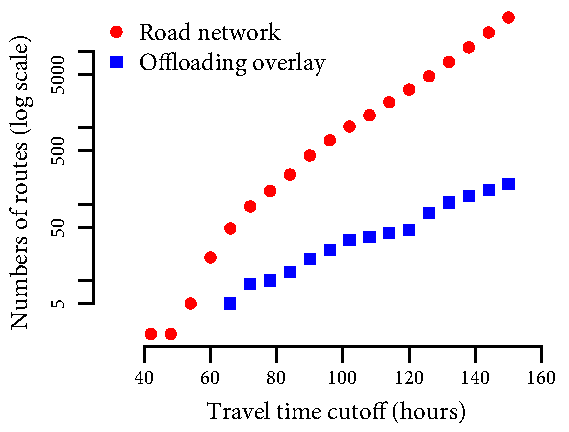
\includegraphics[width=7.2cm]{results/pathcount.pdf}
    \caption{Total number of simple paths in the road network and in the offloading overlay as a function of the travel time cutoff ($y$-axis is in a logarithmic scale).}
    \label{fig:pathcount}
\end{wrapfigure}
For this evaluation, we enumerate all the possible simple paths in both the offloading overlay and the road network. This evaluation shows the benefits of the offloading overlay in mitigating the complexity of the road network. 

We plotted the total number of simple paths bounded by a travel time cutoff in both the road network and the offloading overlay. The plot is represented in Figure~\ref{fig:pathcount} and shows the number of all simple paths as a function of the travel time cutoff of the enumerated paths. In both cases, the number of simple paths grows exponentially with the travel time cutoff. The number of simple paths is much larger on the road network compared to those enumerated in the offloading overlay. Also, the difference in the number of paths grows exponentially. This exponential growth is the main complexity factor to consider when solving the vehicle flow allocation problem.


\subsection{Revenue maximization of offloading data}
\label{sec:res-revenue-max-model}

We interface the offloading overlay we created with \acrshort{cplex} using the linear optimization models we presented in Section~\ref{sec:revenue-maximization-model}. We consider a scenario with the following three different offloading demands (distances are Euclidean) we represent in Figure~\ref{fig:france-demand-allocation-feasibility}:

\begin{itemize}

	\item Offloading demand $d_A$: from Paris to Lyon (384~km).

	\item Offloading demand $d_B$: from Paris to Bordeaux (492~km).

	\item Offloading demand $d_C$: from Paris to Marseille (646~km). 

\end{itemize}

\begin{wrapfigure}[14]{o}[0.7\marginparwidth]{8cm}
    \vspace{-5pt}
    \centering
    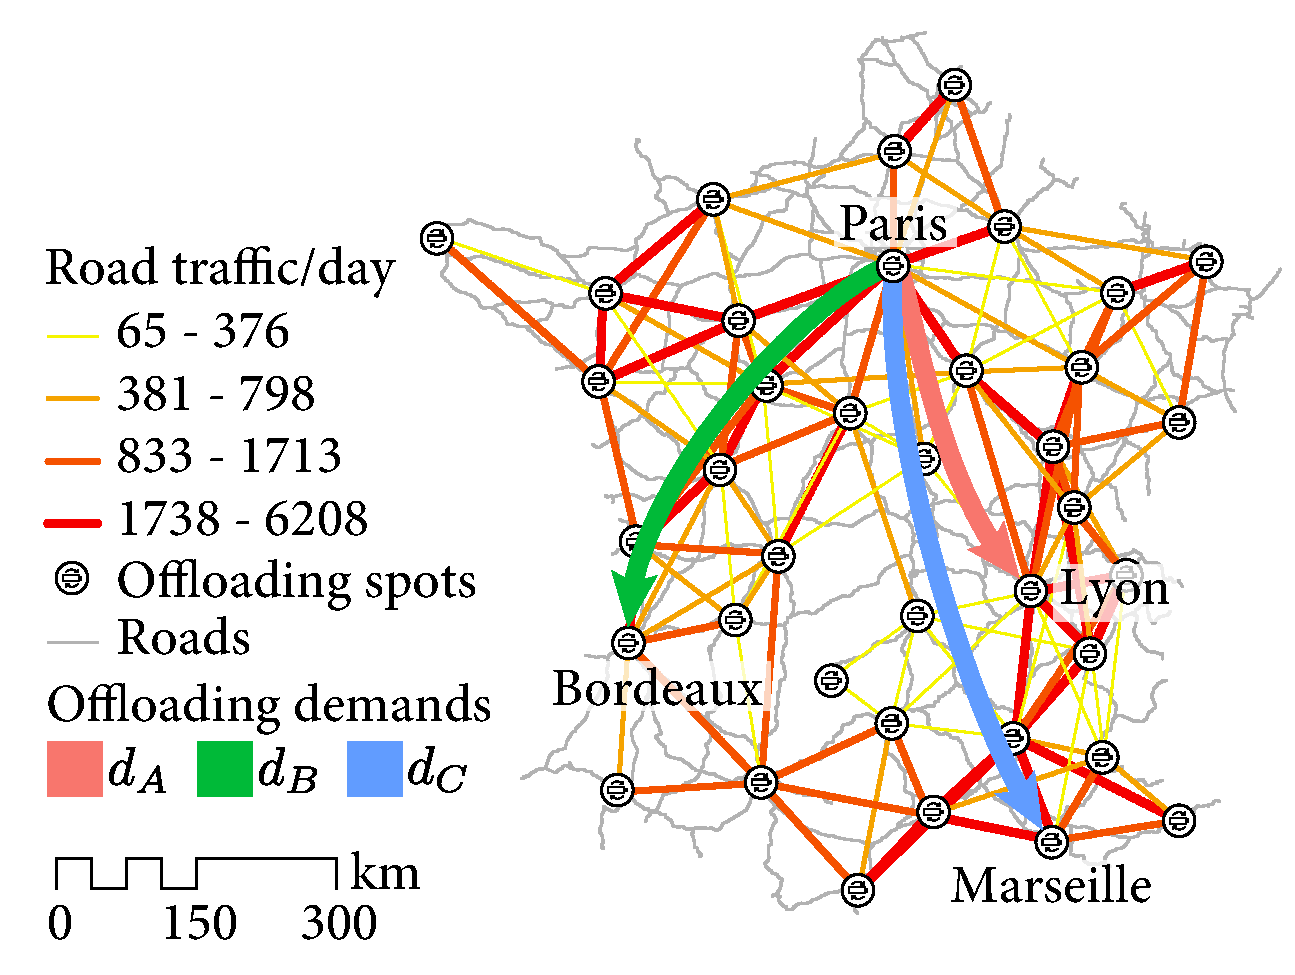
\includegraphics[width=7.8cm]{figures/France-overlay-feasibility.pdf}
    \caption{Schematic representation of the demands $d_A$, $d_B$, and $d_C$.}
    \label{fig:france-demand-allocation-feasibility}
\end{wrapfigure}
It is important to note that demands $d_A$ and $d_C$ will compete for the flows since they share some common subpaths, as we will see in Figure~\ref{fig:allocation-subpaths-offloading-overlay}. This leads to fairness issues, as competing demands will be favored over other demands with the cost-benefit maximization objective, depending on how well they perform. In the following, we discuss how to ensure fairness among the competing flows.

We use a breadth-first search algorithm to generate all the simple logical paths on the offloading overlay for each offloading demand. The cutoffs of the simple paths are given by Equations~\ref{eq:cutoff-rep} and~\ref{eq:cutoff-nrep} for the local replication \textit{rep} and source replication \textit{nrep} models, respectively. However, the generation of the simple logical paths between a source and a destination is exponential, as seen in Figure~\ref{fig:pathcount} of the previous chapter. To solve this issue, we reduce our search space by applying a default cutoff of 12 hours on the travel time of the simple logical paths we generate for our experiments. A 12-hour cutoff is sufficient for each generated path to cover all end-to-end trips within France and small enough to avoid unnecessary path computation.

\begin{wrapfigure}[14]{o}[0.7\marginparwidth]{7.5cm}
    \vspace{-15pt}
    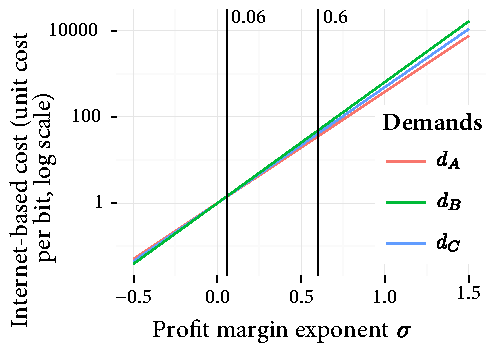
\includegraphics[width=7.2cm]{results/ton-demand-price-km.pdf}
    \caption{Internet-based cost (expressed as the unit cost per bit transferred) as a function of the profit margin exponent for each demand $d_A$, $d_B$, and $d_C$.}
    \label{fig:demand-price-km}
\end{wrapfigure}
We arbitrarily express the Internet-based cost $\gamma_{st}$ as an exponential function of $\text{dist}(s,\,t)$, the distance (in kilometers) between $s$ and $t$:
\begin{equation}
    \gamma_{st} = \big[\text{dist}(s,\,t)\big]^{\sigma}, \text{ where } \sigma\in\mathbb{R}.
\end{equation}
We represent the Internet-based cost $\gamma_{st}$ to transfer a bit of data as a function of the profit margin exponent $\sigma$ for each demand $d_{st}\in\{d_A,\,d_B,\,d_C\}$ in Figure~\ref{fig:demand-price-km}. As shown in the figure, the Internet-based cost increases with the distance (\eg it is greater for the furthest demand $d_C$) for positive values of the profit margin exponent. Note that the Internet-based cost can be adjusted with a factor to account for more realistic prices.

In our experiments, we investigate the impact of the following parameters: the Internet-based cost exponent $\sigma$, the delay tolerance $\tau_{st}$, the leakage tolerance $l_{st}$, and the logical link leakage $l(i,\,j)$ for logical link $(i,\,j)\in L^{O}$. By default, for all the demands, we set leakage tolerance to $10^{-2}$, logical link leakage to 0.05, and delay tolerance to 96~hours (4~days), such that there is enough time for the allocated paths and flows to stabilize (\ie in steady state). The operational costs $\alpha^{\text{rep}}_{i}$ and $\alpha^{\text{nrep}}_{i}$ are weighted by the demands allocated to offloading spot $i$, resulting from the facility-allocation problem. For offloading spot $i$, we set $\alpha^{\text{nrep}}_{i}$ as the normalized weight of the demands allocated to the offloading spot and  $\alpha^{\text{rep}}_{i} = 1,000 \times\alpha^{\text{nrep}}_{i}$. Finally, for each offloading spot $i$, we consider a waiting time $\delta_{i} = 20$ minutes, which corresponds to the duration of a charge that provides a 300~km range to the vehicles (without any queuing time).

% For the sake of clarity, we chose not to show any results on the cost-benefit. 
As our objective is to obtain fair flow allocation, we tune the Internet-based cost exponent $\sigma$ accordingly. The arbitrary choice of $\sigma$ clearly impacts the resulting cost-benefit that can be achieved. That said, different $\sigma$ values lead to different settings for the parameters we consider (delay tolerance, leakage tolerance, and logical link leakage).

We solve the transfer assignment problem from a macroscopic point of view. In this way, we do not have to consider the scheduling problem and the forwarding decisions made at the offloading spots, which both require an analysis on a per-vehicle basis. The results presented in this section are thus achieved under ideal conditions and show an upper-bound of the performance of the offloading. However, to provide more realistic results, we take account of the scheduling and forwarding errors by means of the logical link leakage.

% The results of the evaluation are shown in Fig.~\ref{fig:evaluation}.

\begin{figure*}[!t]
    \centering
    \begin{subfigure}[b]{0.8\textwidth}
        \centering
        
\includegraphics[width=\textwidth]{results/legend.pdf}
    \end{subfigure}%

    \begin{subfigure}[b]{0.50\textwidth}
        \centering
        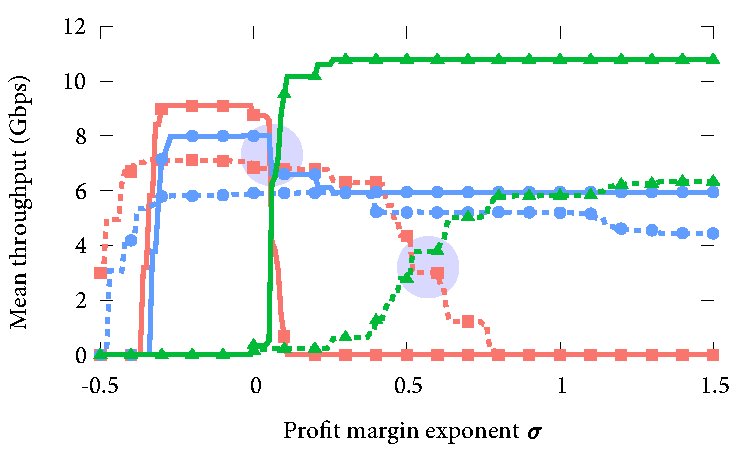
\includegraphics[width=\textwidth]{results/beta-ton.pdf}
        \caption{Throughput as a function of Internet-based cost exponent $\sigma$.}
        \label{fig:ton-beta}
    \end{subfigure}%
    ~ %add desired spacing between images, e. g. ~, \quad, \qquad etc.
      %(or a blank line to force the subfigure onto a new line)
    \begin{subfigure}[b]{0.50\textwidth}
        \centering
        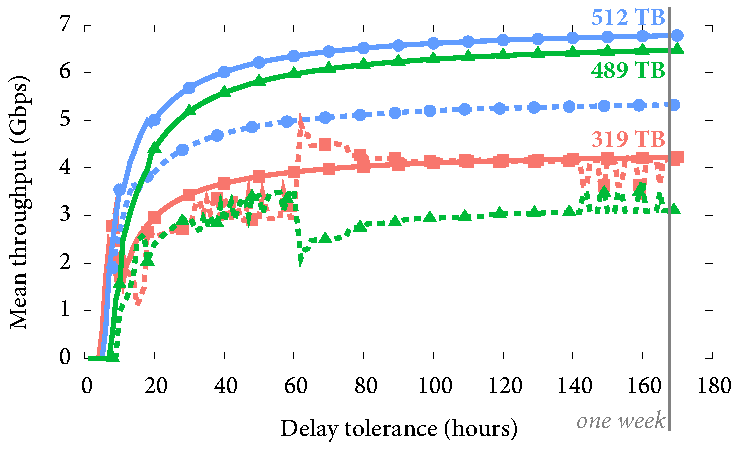
\includegraphics[width=\textwidth]{results/delayTolerance-ton.pdf}
        \caption{Throughput as a function of delay tolerance $\tau_{st}$.}
        \label{fig:ton-delayTolerance}
    \end{subfigure}
    
    \begin{subfigure}[b]{0.50\textwidth}
        \centering
        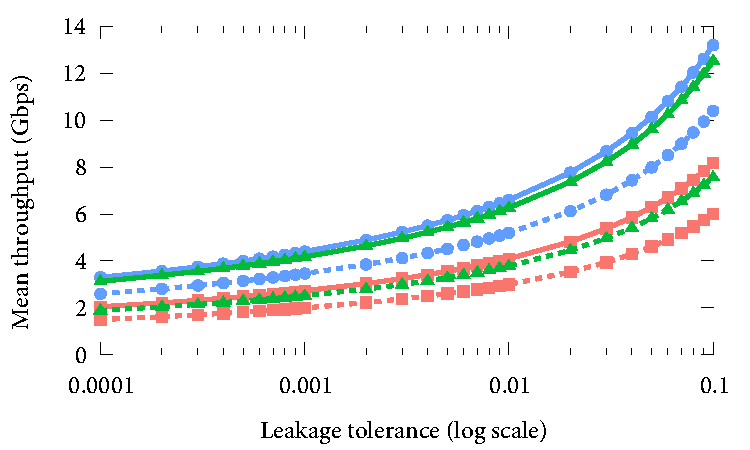
\includegraphics[width=\textwidth]{results/leakageTolerance-ton.pdf}
        \caption{Throughput as a function of leakage tolerance $l_{st}$.}
        \label{fig:ton-leakageTolerance}
    \end{subfigure}%
    ~ %add desired spacing between images, e. g. ~, \quad, \qquad etc.
      %(or a blank line to force the subfigure onto a new line)
    \begin{subfigure}[b]{0.50\textwidth}
        \centering
        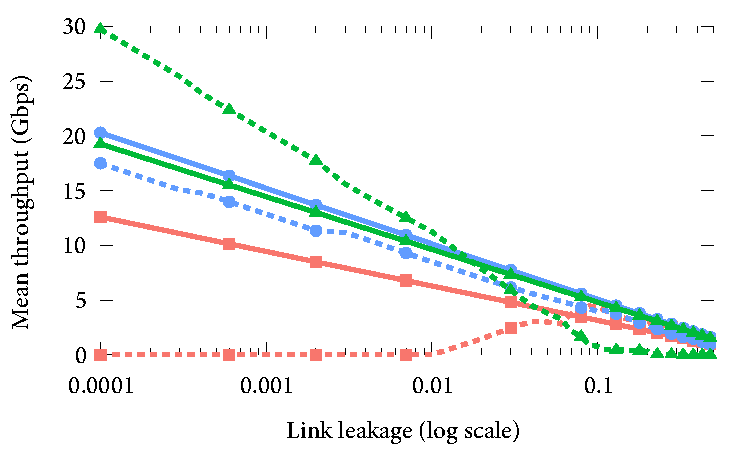
\includegraphics[width=\textwidth]{results/linkLeakage-ton.pdf}
        \caption{Throughput as a function of logical link leakage $l(i,\,j)$.}
        \label{fig:ton-linkLeakage}
    \end{subfigure}
    \caption{Evaluation results with, by default, delay tolerance $\tau_{st} = 96$~hours, leakage tolerance $l_{st} = 0.01$, logical link leakage $l(i,\,j) = 0.05$ for all offloading demands $d_{st}$. The values of the Internet-based cost $\sigma^{\text{rep}}$ and $\sigma^{\text{nrep}}$ are chosen such that the standard deviation of the throughput of all flows is minimized, to ensure fairness among competing data offloading demands.}
    \label{fig:ton-evaluation}
\end{figure*}

In Figure~\ref{fig:ton-evaluation}, we first note that the \textit{rep} model (with solid lines) always achieves better throughputs than the \textit{nrep} model (with dashed lines). Indeed, the \textit{nrep} model takes into account all logical link leakages in the paths it considers and replicates the data accordingly, sending more data than the \textit{rep} model. We also note that our offloading infrastructure can achieve transfers with a throughput above 10~Gbps and aggregated data transfers in the Petabyte range with the \textit{rep} model within a week (\ie as shown in Figure~\ref{fig:ton-delayTolerance}: 512~TB transferred within a week for demand $d_B$, 489~TB for $d_C$, and 319~TB for $d_A$ amounts to 1,320~TB transferred within a week).

Figure~\ref{fig:ton-beta} represents the evolution of the throughput of the three demands as a function of $\sigma$, given the delay tolerance, the leakage tolerance, and the logical link leakage. We note that the value of $\sigma$ is decisive concerning the allocation of the flows to favor: either short distance (demand $d_A$) or long distance (demands $d_B$ and $d_C$). This behavior happens in both \textit{rep} and \textit{nrep} models, although the breaking points (represented by circles in the plot) are not the same for the two models: the break happens at $\sigma = 0.06$ for the \textit{rep} model, and $\sigma = 0.6$ for the \textit{nrep} model. Beyond these points, long-distance demands are favored compared with short-distance ones. Indeed, $\gamma_{st}$ is a factor in the maximization objective (defined in Section~\ref{sec:revenue-maximization}) and the higher the $\gamma_{st}$, the bigger the total revenue we aim to maximize. As shown in Figure~\ref{fig:demand-price-km}, since $\sigma$ is the exponent of the Euclidean distance between $s$ and $t$, we have:

\begin{itemize}

	\item If $\sigma < 0$, $\gamma_{st}$ decreases when the distance increases, favoring short-distance offloading demands.

	\item If $\sigma = 0$, $\gamma_{st} = 1$, favoring short-distance demands with a lower average travel time between the source and destination.

	\item If $\sigma > 0$, $\gamma_{st}$ increases with the distance, favoring long-distance offloading demands.

\end{itemize}

Although the impact of $\sigma$ on the allocation of the flows between demands $d_A$ and $d_C$ is strong, the impact is weaker with demand $d_B$, as this latter shares few subpaths with $d_A$ and $d_C$, as represented in Figure~\ref{fig:allocation-subpaths-offloading-overlay}. Since we want a fair flow allocation when offloading data, we choose $\sigma^{\text{rep}}$ and $\sigma^{\text{nrep}}$ such that the standard deviation of the throughput of all flows is minimized.

It is important to keep in mind, however, that this allocation has an impact on the total revenue because $\gamma_{st}$ is the factor that generates the revenue. Since $\sigma^{\text{rep}} < \sigma^{\text{nrep}}$, the \textit{nrep} model has a revenue that is much larger than the \textit{rep} model. 

\begin{wrapfigure}[13]{o}[0.7\marginparwidth]{6cm}
    \vspace{-15pt}
    \centering
    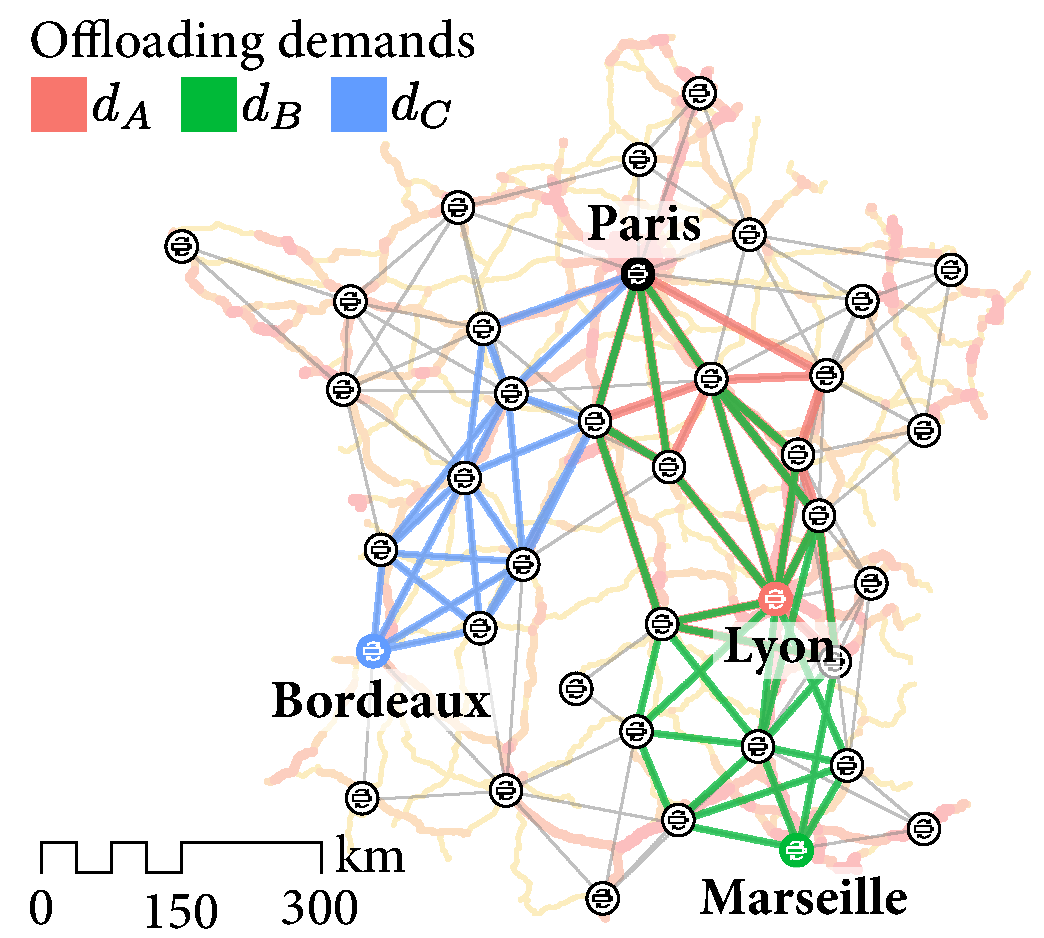
\includegraphics[width=5.4cm]{figures/France-AADT-overlay-layers.pdf}
    \caption{Representation of the logical paths allocated to the three demands $d_A$, $d_B$, and $d_C$.}
    \label{fig:allocation-subpaths-offloading-overlay}
\end{wrapfigure}
Figure~\ref{fig:ton-delayTolerance} shows the throughput as a function of the delay tolerance $\tau_{st}$ (\ie the total duration of the transfer). We notice that the throughput stabilizes as the duration of the transfer increases. For the \textit{rep} model (solid lines), demands with longer distances are favored (demand $d_B$ and $d_C$) over demands with shorter distances (demand $d_A$) Indeed, the total revenue is increased when favoring demands with longer distances, as seen on Figure~\ref{fig:ton-beta}. For the \textit{nrep} model (dashed lines), the allocation of demands $d_A$ and $d_C$ oscillates, favoring one or the other. Both demands have flows allocated on shared subpaths, depending on the maximization of the total revenue. The oscillation results from the variation of the value of $\sigma^{\text{nrep}}$, which depends on the minimization of the standard deviation of the throughput of the allocated flows.

\begin{wrapfigure}[14]{o}[0.7\marginparwidth]{8.5cm}
    \centering
    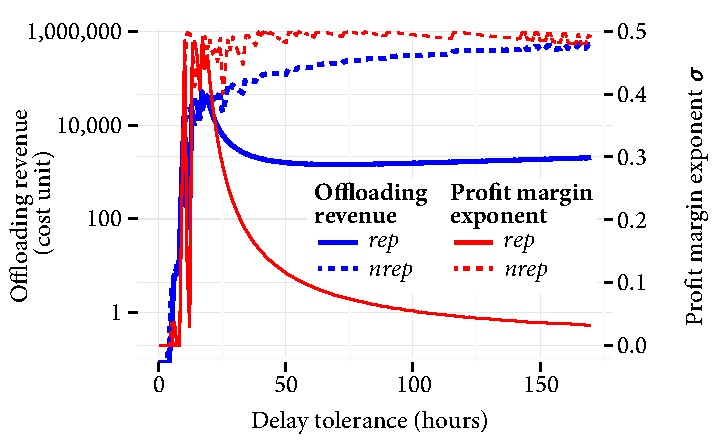
\includegraphics[width=8.2cm]{results/revenue-delaytolerance.pdf}
    \caption{Offloading revenue as a function of the delay tolerance resulting from the allocation of demands $d_A$, $d_B$, and $d_C$, respective to Figure~\ref{fig:ton-delayTolerance}.}
    \label{fig:revenue-delay-tolerance}
\end{wrapfigure}
We represent the offloading revenue (in terms of cost unit) for the allocations of demands $d_A$, $d_B$, and $d_C$ (respective to Figure~\ref{fig:ton-delayTolerance} as a function of the delay tolerance of the offloading demands. Note that the revenue depends on the Internet-based cost and the profit margin exponent $\sigma$. Recall that the latter is chosen for each allocation of the demands given a delay tolerance to guarantee fair allocation of the demands, such that it minimizes the standard deviation of the mean throughput resulting from the allocation of the demands. For this reason,  the resulting offloading revenue is unstable for small delay tolerances (\ie < 50 hours). When increasing the delay tolerance of the offloading demands, the profit margin decreases to guarantee the fairness of the allocations of the demands and the revenue increases. Since more data is transferred, the revenue is becoming less sensitive to the transfer distances and $\sigma$ decreases. Additionally, the revenue resulting from the \textit{rep} model is less than the \textit{nrep} model, as the operational costs when traversing the offloading spots are 1,000 times less for the \textit{nrep} model (since it requires less data to be stored temporarily due to replications).

Finally, Figures~\ref{fig:ton-leakageTolerance} and~\ref{fig:ton-linkLeakage} show the throughput as a function of, respectively, the leakage tolerance $l_{st}$ and logical link leakage $l(i,\,j)$.  The throughput increases when the leakage tolerance increases or the logical link leakage decreases. The \textit{nrep} model almost achieves the same performance, if not better, than the \textit{rep} model when there is a low logical link leakage ($l(i,\,j) < 0.05$). The logical link leakage also has an effect on the allocation of the flows for the \textit{nrep} model when the flows share subpaths, contrary to the \textit{rep} model: shorter distances (demand $d_A$) are favored with a high logical link leakage ($\mathcal{L}(i,\,j) > 0.05$) and longer distances (demands $d_B$ and $d_C$) are favored with a low logical link leakage ($l(i,\,j) < 0.05$). Indeed, the objective function of the \textit{nrep} model depends on the multiplied logical link leakage $l_{p}(i,\,j)$.


\section{Discussion}
\label{sec:discuss}

\subsection{Data security}

The owners of the electric vehicles may try to access the data payload they are carrying. Therefore, the data has to be encrypted so that only the content provider is able to read it. For instance, a public-key infrastructure can be considered (\eg RSA, ECC). The data is encrypted with the public key of the remote entity (the destination of the data) by the originating entity (the source of the data) and will be in turn decrypted by the remote entity using their private key. Also, we can use certificates to authenticate the originating entity of the data by the remote entity.  

Also, we consider a multiple path allocation of the data both on the road infrastructure and on the offloading overlay, which offers path diversity. Therefore, the data that is part of the same flow (or even the same data when replicated) will not take the same path (either road path or logical path). This provides robustness for data transfers, as well as increased security since the data belonging to the same flow will be scattered over multiple paths, making it difficult to attack the whole data transfer by preventing single vantage point attacks.

\subsection{Drayage system}

Recall that data is offloaded from a conventional data network to the closest offloading spot using a drayage system\index{drayage|bb}. The drayage is equivalent to the first and last mile of the access networks in an Internet-based transfer. The drayage can be carried out by different means:

\begin{itemize}
    
    \item \textit{Dedicated lines} (\eg optical fiber channels) can be set up between the different locations that need drayage. This solution would be adapted to connect locations that require continuous large data exchanges. However, it does not fit temporary data exchanges, as it is a costly solution (\eg the sources and destinations of a data transfer are only temporary). 

    \item \textit{Dedicated vehicles} can provide data drayage between the different locations. These vehicles would be equipped with storage and communication capabilities, with the data size and rates greater in magnitude than the common vehicles we consider in this thesis.

\end{itemize}


\subsection{Predicting the future direction of the stopping vehicles and privacy concerns}

For each stopping vehicle, the offloading spot must determine the subsequent offloading spot on the vehicle's route. The offloading service provider stores \textit{anonymously} the previous locations of the vehicles in a historical database to help the offloading spots predict the remaining itinerary of the stopping vehicles. To this end, the service provider can use probabilistic tools, such as Hidden Markov Models~\cite{simmons2006learning}, maximum entropy~\cite{ziebart2008maximum}, or Bayesian networks~\cite{liao2007learning,krumm2006predestination}. The partial trajectories of the vehicles can be known through the successive locations recorded by the navigation system of the vehicles. Note that, the current road traffic in the vicinity of the offloading spot can also help predict the most likely routes vehicles will take~\cite{xue2009traffic}. 

In order to \textit{accurately} predict the future offloading spot the vehicle will visit, the offloading service requires access to the positioning data of the vehicles, which raises some privacy concerns. While it is common for car manufacturers to collect and analyze such data (\eg Tesla collects the current location of the vehicles for remote vehicle analysis\footnote{https://www.tesla.com/about/legal}), we are aware of the privacy breach this represents for both the driver and passengers. In Section~\ref{sec:business-model}, we presented a ``get paid to drive'' program offered by the offloading service provider to the vehicle owners in exchange for transporting a storage device. With this incentive, some drivers may be more willing to share their positioning data with the service.  Otherwise, the offloading service provider could use the historical visit of the vehicle at charging stations (operated by the charging station operator) to infer the vehicles' future visits based on probabilistic tools (\eg Markov chains).

When the drivers do not want to share any data at all with the offloading service, the offloading spots discard the vehicles that do not share their positioning data because there is no means to predict where they will go next. In this case, these vehicles should not be involved in the data offloading.

\section{Conclusion}
\label{sec:revenue-maximization-conclusions}

In this chapter, we presented the concept of offloading data traffic onto the road network. This concept exploits the existing mobility of vehicles to extend the capacity of conventional data networks such as the Internet. We assessed this concept by comparing the cost of using the road network to transfer data with the cost of transferring the same amount of data on the Internet. To determine the road path providing similar performance in terms of delay and bandwidth as in the case of the Internet, we proposed an allocation model that maximizes the cost-benefit of offloading traffic on the road network over conventional data transfers. To solve this model in reasonable computational time, we proposed a road map reduction procedure which produces a simplified logical representation of the road network.  
%We used data replication the offloading spots to provide reliable data transfers. 
We evaluated this allocation model on the main roads of France using actual road traffic counts. Our results show that the road network can accommodate simultaneous data transfers with an aggregate capacity in the Petabyte range per week.

% In this chapter, we character defined the revenue maximization problem that maximizes the cost-benefit achieved by the offloading service content providers offload data transfers on the road network compared to the use of infrastructure-based networks. We then devise two models derived from two data replication strategies at the offloading spots. With the first replication strategy \textit{rep}, each offloading spot on the allocated logical paths of the data transfers replicates data on multiple vehicles. With the second replication strategy \textit{nrep}, the data is replicated at the source of the transfer and no data is replicated at the intermediate offloading spots. In both cases, the amount of data to replicate at the offloading spots depends on the logical link leakage and it achieved such that the leakage tolerance of the offloading demands is satisfied. We evaluated each of the revenue maximization models on the road network of France. Our offloading service allows data transfers in the Petabyte range per week with a market share of 20\% and only one Terabyte of storage per vehicle. These results confirm the offloading potential of our service, which can help operators handle large amounts of data.